% ----------------------------------------------------------------------------------------------------
% V 3.0 
% - V.2.2: Revised shortened version
% - V.2.3: Modified tone and dropped HYPOTHESIS type statements
% - V.3.0: 15-Jul -- Add NEW results 
% - V.4.0: 18-Jul -- Add 17-Jul results. Added model size.
% ----------------------------------------------------------------------------------------------------

\PassOptionsToPackage{hypertexnames=false}{hyperref}
\documentclass[sn-basic]{sn-jnl}% Basic Springer Nature Reference Style (local sn-basic.bst available)

%% Standard Packages
\usepackage{caption}
\usepackage{subcaption}
\usepackage{graphicx}%
\usepackage{pgfplots}
\pgfplotsset{compat=1.18}
\usepackage{multirow}%
\usepackage{amsmath,amssymb,amsfonts}%
\usepackage{amsthm}%
\usepackage{mathrsfs}%
\usepackage[title]{appendix}%
\usepackage{textcomp}%
\usepackage{manyfoot}%
\usepackage{setspace}
\usepackage[table]{xcolor}
\usepackage{booktabs}
\usepackage{array}

\graphicspath{{figures/}}

% --- MACRO DEFINITION ---
\newcommand{\faintcmidrule}[1]{%
	\arrayrulecolor{black!30}%
	\cmidrule{#1}%
	\arrayrulecolor{black}%
}

\newcolumntype{L}[1]{>{\raggedright\arraybackslash}p{#1}}

% % % Usage: \faintcmidrule{2-4} % Optional thickness: \faintcmidrule[0.2pt]{2-4}
% \newcommand{\faintcmidrule}[2][0.25pt]{%
%   \cmidrule[#1](lr){#2}%
% }

\graphicspath{{figures/}}

\makeatletter
\def\toclevel@paragraph{3}
\def\toclevel@subparagraph{4}
\makeatother

\onehalfspacing
\renewcommand{\arraystretch}{1.44}
% \lstset{
%         basicstyle=\ttfamily\footnotesize,
%         columns=fullflexible,
%         breaklines=true,
%         frame=single,
%         xleftmargin=0.5em,
%         xrightmargin=0.5em,
%         aboveskip=0.8em,
%         belowskip=0.8em
% }

\begin{document}

\title[RL for PdM]{Reinforcement Learning for Predictive Maintenance: A study of Attention Mechanisms for Milling Tool Replacement (2.3)}

\author[1,4]{\fnm{Rajesh} \sur{Siraskar} \sfx{(\href{https://orcid.org/0000-0003-2341-8787}{ORCID: 0000-0003-2341-8787}})}\email{rajesh.siraskar@gmail.com}
\author*[1,2]{\fnm{Satish} \sur{Kumar}}\email{satish.kumar@sitpune.edu.in}
\author[1,2]{\fnm{Shruti} \sur{Patil}}
\author[1]{\fnm{Arunkumar} \sur{Bongale}}
\author[1,2]{\fnm{Ketan} \sur{Kotecha}}
\author[3]{Ambarish Kulkarni}


\affil*[1]{\orgdiv{Symbiosis Institute of Technology}, \orgname{Symbiosis International (Deemed University)}, \orgaddress{\city{Pune}, \postcode{412115}, \state{Maharashtra}, \country{India}}}
\affil[2]{\orgdiv{Symbiosis Centre for Applied Artificial Intelligence}, \orgname{Symbiosis International (Deemed University)}, \orgaddress{\city{Pune}, \postcode{412115}, \state{Maharashtra}, \country{India}}}
\affil[3]{Swinburne University of Technology, Hawthorn VIC 3122, Australia}
\affil[4]{\orgdiv{CTO Office}, \orgname{Birlasoft Ltd.}, \orgaddress{\city{Pune}, \postcode{411057}, \state{Maharashtra}, \country{India}}}

\abstract{Predictive maintenance helps decide when a machine component should be replaced before failure. This paper studies milling cutting-tool replacement. The decision is asymmetric: late replacement can affect quality or cause failure, while early replacement wastes tool life. We model this as a Reinforcement Learning (RL) problem and test whether \textsc{REINFORCE}, a Monte-Carlo policy-gradient method, remains competitive with common RL baselines.

We compare \textsc{A2C}, \textsc{DQN}, \textsc{PPO}, and \textsc{REINFORCE} with four attention-style feature extractors: Nadaraya--Watson, temporal, multi-head, and self-attention. We also add a no-attention ablation, where the normalized sensor vector is passed directly to the policy. The experiments use a Gymnasium-compatible milling environment and an AutoRL workflow for training and reporting.

The method is evaluated on the public IEEE PHM~2010 milling dataset and an in-house university testbed dataset. In both schemas, the no-attention baseline winner is \textsc{PPO} (SIT: 0.6313, IEEE: 0.8434), while the best model with attention is \textsc{REINFORCE} (SIT: 0.7492, IEEE: 0.8569). For the focused comparison \textsc{REINFORCE} $>$ \textsc{PPO}, baseline differences are not supported (SIT: $t=-2.9224$, $p=0.9980$; IEEE: $t=-1.3711$, $p=0.9100$), but with attention the claim is supported (SIT: $t=3.1941$, $p=0.0007$; IEEE: $t=1.9865$, $p=0.0243$). Ablation results support attention interoperability across schemas for \textsc{REINFORCE}: attention significantly improves over the no-attention baseline in both SIT (0.4907 to 0.7492, $p=0.0000$) and IEEE (0.7496 to 0.8569, $p=0.0440$).}

\keywords{Predictive maintenance, Industry 4.0, Reinforcement Learning, REINFORCE, Attention mechanisms, Ablation study, Milling, AutoRL}

\maketitle

\section{Introduction}
\subsection{Background}
Predictive maintenance (PdM) tries to replace or service a component before failure, while still using useful life effectively. Modern machines generate sensor data during operation, and this data can support maintenance decisions \cite{Zonta2020, Compare2020}. In milling, the cutting tool wears gradually. Since direct wear inspection usually interrupts machining, a practical method should use signals already available during cutting.

\subsection{Problem statement}
This paper studies a direct PdM question: when should a milling cutting tool be replaced? Late replacement can lead to defective parts or tool failure. Early replacement is safer, but wastes tool life and interrupts production. RL is a natural fit because the agent repeatedly chooses between two actions: replace or continue.

The main research question is: \emph{Can \textsc{REINFORCE} remain competitive with commonly used RL methods such as \textsc{DQN}, \textsc{A2C}, and \textsc{PPO} for milling PdM when it is paired with attention-based feature extraction, and does attention improve over a no-attention observation baseline?}

\subsection{Contributions}

This study builds on our earlier work on \textsc{REINFORCE} for PdM \cite{Siraskar2025} and on our prior use of Nadaraya--Watson attention for tool-wear prediction \cite{Siraskar2024}. Here, AutoRL gives a common workflow for training, evaluation, and reporting across algorithms, hyperparameters, and feature extractors \cite{Schwartz2020, Strubell2019, Faust2019, Mussi2022}.

\textbf{Research objectives and hypotheses:}
The objectives are to compare RL algorithms for milling PdM, test whether \textsc{REINFORCE} is competitive, evaluate attention against no-attention baselines, use one Gymnasium-compatible environment across two schemas, and report the results through the same AutoRL workflow.

We test three research themes:
\begin{itemize}
    \item \textbf{REINFORCE:} For the given predictive maintenance task for a milling machine tool replacement -- how does the light weight \textsc{REINFORCE} algorithm perform in comparison with more advanced algorithms such as \textsc{A2C}, \textsc{DQN}, and \textsc{PPO}. This is a continued research theme from \cite{Siraskar2025}.
    \item \textbf{Attention mechanisms:} How do attention based feature extractors affect RL agorithm \textsc{REINFORCE} performance and improve over a matched no-attention baseline in at least some schema--mechanism settings.
	\item \textbf{H2:} The same Markov Decision Process (MDP), environment design, and reward logic can be used on two different milling-machine schemas (SIT\footnote{Symbiosis Institute of Technology} and IEEE), without claiming direct transfer of a trained policy from one schema to the other.
  
\end{itemize}

\textbf{Contributions:}
This paper contributes:
\begin{itemize}
    \item \textbf{RL comparison:} \textsc{REINFORCE}, \textsc{A2C}, \textsc{DQN}, and \textsc{PPO} are compared on a milling tool-replacement task.
    \item \textbf{Attention ablation:} four attention-style extractors are compared with matched no-attention baselines.
    \item \textbf{Schema-aware environment:} one Gymnasium-compatible environment is used with both SIT and IEEE sensor schemas.
    \item \textbf{AutoRL workflow:} raw sensor readings, model selection, checkpointing, and reporting are handled in one workflow.
\end{itemize}

\section{Literature Review and Technical Background}
\label{sec:lit_tech}
\subsection{PdM and industrial decision-making}
PdM connects sensing, analytics, and maintenance decisions in production systems \cite{Compare2020, Zonta2020}. Prescriptive maintenance extends this by recommending an action, such as replace or continue \cite{Ansari2019}. In manufacturing, such recommendations are useful only when they can be linked to signals available on the machine.

\subsection{RL for predictive maintenance}
RL has been studied for maintenance scheduling, inspection planning, and condition-based maintenance \cite{Siraskar2023, Ogunfowora2023, Zhang2024}. Simpler RL formulations are often useful when the state and action spaces are structured \cite{Adsule2020, Yousefi2020, Rasay2024, Dadash2024}. Deep RL methods, such as DQN and PPO, are common when observations or horizons are more complex \cite{Liu2020, Chen2023, Lee2022, Ong2022-02}. Recent review work also notes that \textsc{REINFORCE} has received less PdM attention than these methods \cite{Siraskar2025}.

Public PdM benchmarks are useful, but they do not capture all plant-specific degradation, sensors, and maintenance rules. Evidence from physical manufacturing systems therefore remains important \cite{Andrade2021Aircraft,Dangut2022RareFailure,Chen2024DigitalTwin}. Attention-based models may also depend on the sensor structure of the machine being studied \cite{Zhao2024}. This motivates testing both the public IEEE data and the in-house SIT data.

\subsection{Technical background: MDP setting and RL algorithms}
\label{sec:tech_background}
\paragraph{MDP notation and observation model:}
We model milling PdM as an episodic MDP $(\mathcal{S},\mathcal{A},P,R,\gamma)$, where the agent observes sensor state $s$, takes action $a$, receives reward $R$, and moves according to $P$. Section~\ref{sec:env} applies this form to tool replacement.

\paragraph{RL algorithms compared:}
We compare DQN, A2C, PPO, and \textsc{REINFORCE} using the same environment and observation interface \cite{Mnih2015, Schulman2017, Williams1992}.

\section{Materials and Methods}
\label{sec:method}

\subsection{Problem formulation: RL for PdM with attention}
\label{sec:env} \label{app:env_reward}
\paragraph{Milling machines:}
Milling tools gradually wear during machining and are replaced near the end of useful life. We use $\tau = 300\,\mu\mathrm{m}$, as suggested in Section 7.4 of ISO 8688-2:1989 \citep{ISO8688-2-1989}, as the wear threshold for training, reward shaping, and evaluation.

At each decision step $t$, the agent selects $a_t\in\{0,1\}$, where $a_t=0$ means \emph{replace} and $a_t=1$ means \emph{continue}. Replacement ends the episode; continuing keeps the process running.

True wear is not available online because it requires inspection. The agent therefore uses in-process sensor data $\mathbf{x}_t\in\mathbb{R}^d$. Measured wear is used inside the environment only for threshold checks, termination, and rewards.

\paragraph{Attention as representation learning for sensor-driven PdM:}
Because decisions use $\mathbf{x}_t$ rather than direct wear inspection, each RL algorithm is paired with an attention-style extractor $\phi_\theta(\mathbf{x}_t)$ before the policy/value network.

\subsection{State space, action space, and reward function}
\label{sec:mdp_components}

\paragraph{State space (observation model):}
The information state is the sensor vector $\mathbf{x}_t$. The two schemas differ in sensors and channel count (Table~\ref{tab:schema_features}), but the decision meaning is fixed.

\paragraph{Dataset schemas and observation channels:}
\begin{table}[htbp]
\centering
\caption{Sensor channels used as observations by the RL environment}
\label{tab:schema_features}
	\begin{tabular}{L{0.18\linewidth} L{0.75\linewidth}}
	\toprule
	\textbf{Schema} & \textbf{Observation channels}\\
	\midrule
	SIT & Spindle vibration, table vibration, spindle sound, table sound, load-cell ($x$/$y$/$z$), spindle current\\
	IEEE & Cutting force ($x$/$y$/$z$), vibration ($x$/$y$/$z$), acoustic-emission RMS\\
	\bottomrule
	\end{tabular}
\end{table}

\paragraph{Action space:}
The action space is discrete: $a_t=0$ means \emph{replace}, and $a_t=1$ means \emph{continue}.

\paragraph{Reward function and PdM asymmetry:}
PdM decisions are asymmetric. Late replacement may cause quality loss or failure; early replacement wastes useful life. The reward therefore encourages safe use, penalizes threshold violations, and rewards replacement near $\tau$.

\begin{table}[htbp]
	\centering
	\caption{Conceptual interpretation of PdM decisions}
	\label{tab:cost_view}
	\begin{tabular}{L{0.18\linewidth} L{0.32\linewidth} L{0.42\linewidth}}
		\toprule
		\textbf{Case} & \textbf{Condition} & \textbf{PdM interpretation}\\
		\midrule
		Timely replace & $a_t=0$ near $VB\approx\tau$ & Desired: high utilization and low violation risk.\\
		Early replace & $a_t=0$ when $VB\ll\tau$ & Safe but wasteful: reduces risk while discarding useful life.\\
		Late action / violation & $a_t=1$ while $VB>\tau$ & Worst case: elevated risk of quality loss or failure; strongly penalized.\\
		Continue safely & $a_t=1$ with $VB<\tau$ & Encouraged: extracts remaining useful life when safe.\\
		\bottomrule
	\end{tabular}
\end{table}

\paragraph{Reward shaping components:}
\begin{table}[htbp]
	\centering
	\caption{Reward shaping components in the milling PdM environment (qualitative summary).}
	\label{tab:reward_components}
	\begin{tabular}{L{0.20\linewidth} L{0.22\linewidth} L{0.50\linewidth}}
		\toprule
		\textbf{Component} & \textbf{Applied when} & \textbf{Effect}\\
		\midrule
		$R_1$ survival reward & Continue and safe & Encourages utilization while below threshold.\\
		$R_2$ violation penalty & Violated wear threshold and continued & Strongly discourages threshold violation.\\
		$R_3$ replacement cost & Replace action & Regularizes against replacing too early.\\
		$R_4$ near-threshold bonus & Replace near $\tau$ & Rewards timely replacement close to threshold.\\
		Stepwise bonuses & Wear ratio $\,\ge 0.7, 0.8, 0.9$ & Increases incentive as wear approaches threshold.\\
		\bottomrule
	\end{tabular}
\end{table}

\subsection{Execution implementation: learning pipeline and attention mechanisms}\label{sec:algo_desc}
\paragraph{AutoRL workflow:}\label{sec:autorl}
The AutoRL pipeline runs training, evaluation, and reporting for each algorithm, hyperparameter setting, and feature extractor. Checkpoints allow long runs to resume.

\paragraph{Simulation environment (Gymnasium-compatible milling PdM):}
We define a Gymnasium-compatible environment for milling-tool replacement \cite{Foundation2023}. Episode structure, actions, and reward logic are fixed; only the observation channels vary by schema.

\paragraph{Training procedure and policy architecture:}
All agents are trained using Stable-Baselines3 and a Gymnasium-compatible wrapper. Learning rate $\eta$ and discount factor $\gamma$ are swept because they are shared across algorithms and strongly affect performance \cite{Henderson2019, Shala2022AutoRL, Eimer2023}.
  
\paragraph{Attention mechanisms as feature extractors:}
\label{sec:attention}

Attention mechanisms are used as feature extractors $\phi(\mathbf{x}_t)$. They map the sensor vector into a 64-dimensional embedding for the policy/value networks. Here, ``attention'' means feature reweighting, gating, or structured fusion of the current sensor vector. Temporal context is added only through explicit positional encoding.

For the ablation study, the normalized sensor vector is also passed directly to the policy/value network as a no-attention baseline.

\paragraph{Nadaraya--Watson attention}
Nadaraya--Watson (NW) attention works as kernel-based soft retrieval from learnable prototypes. We include it because it performed well in our earlier PdM attention work \cite{Siraskar2024}.

A standard Gaussian-kernel form is
\begin{equation}
        \mathbf{q}=W_q\mathbf{x}_t,\qquad
        \alpha_i = \frac{\exp\left(-\beta\,\lVert \mathbf{k}_i-\mathbf{q}\rVert^2\right)}{\sum_j \exp\left(-\beta\,\lVert \mathbf{k}_j-\mathbf{q}\rVert^2\right)},
        \qquad \mathbf{z}=\sum_i\alpha_i\,\mathbf{v}_i.
\end{equation}
We use learnable prototypes $\{\mathbf{k}_i,\mathbf{v}_i\}$ and bandwidth $\beta>0$.

\paragraph{Temporal attention}
Temporal attention (TP) adds a stage-of-life signal using sinusoidal positional encodings and a learnable temporal embedding \cite{Vaswani2017, Lim2020TFT}. It combines soft feature reweighting with a timestep encoding:
\begin{align}
        \boldsymbol{\alpha}_t &= \mathrm{softmax}\!\left(W_2\tanh\!\left(W_1\mathbf{x}_t\right)\right),
        \qquad \tilde{\mathbf{x}}_t = \mathbf{x}_t\odot\boldsymbol{\alpha}_t,\\
        \mathrm{PE}(t,2i) &= \sin\!\left(\frac{t}{{T_{max}}^{2i/d_{\mathrm{TP}}}}\right),
        \qquad \mathrm{PE}(t,2i+1)=\cos\!\left(\frac{t}{{T_{max}}^{2i/d_{\mathrm{TP}}}}\right),\\
        \mathbf{e}_t &= \mathrm{PE}(t) + \mathbf{b},
        \qquad \mathbf{z}_t = f_\theta\!\left([\tilde{\mathbf{x}}_t;\mathbf{e}_t]\right).
\end{align}
Here $t$ is the within-episode timestep, $T_{max}$ is the truncation limit, $d_{\mathrm{TP}}$ is the encoding dimension, and $f_\theta(\cdot)$ gives the feature embedding.

\paragraph{Multi-head attention}
Multi-head attention (MH) gates the single-timestep feature vector in parallel subspaces \cite{Vaswani2017}. The heads operate on projections of the current observation, not on a token sequence.

In our implementation,
\begin{align}
        \mathbf{Q}&=W^Q\mathbf{x}_t,\quad \mathbf{K}=W^K\mathbf{x}_t,\quad \mathbf{V}=W^V\mathbf{x}_t,\\
        \mathbf{q}_h&=\mathrm{split}_h(\mathbf{Q}),\quad \mathbf{k}_h=\mathrm{split}_h(\mathbf{K}),\quad \mathbf{v}_h=\mathrm{split}_h(\mathbf{V}),\\
        s_h&=\frac{\mathbf{q}_h^\top\mathbf{k}_h}{\sqrt{d_h}},\quad \alpha_h=\mathrm{softmax}(s)_h,\\
        \mathbf{z}&=W^O\,[\alpha_1\mathbf{v}_1;\ldots;\alpha_H\mathbf{v}_H].
\end{align}

\paragraph{Self-attention}
Self-attention (SA) is applied to the current observation vector. It is therefore a gated feature block with residual connections and layer normalization, not sequence self-attention over a time window.

In our implementation,
\begin{align}
        \mathbf{x} &= W_{\mathrm{in}}\mathbf{x}_t,\\
        \mathbf{q} &= W_Q\mathbf{x},\quad \mathbf{k}=W_K\mathbf{x},\quad \mathbf{v}=W_V\mathbf{x},\\
        s &= \frac{\mathbf{q}^\top\mathbf{k}}{\sqrt{d}},\quad \tilde{\mathbf{x}} = g(s)\,\mathbf{v},\\
        \mathbf{z}_1 &= \mathrm{LN}\!\left(\mathbf{x}+\tilde{\mathbf{x}}\right),\quad
        \mathbf{z}=\mathrm{LN}\!\left(\mathbf{z}_1+\mathrm{FFN}(\mathbf{z}_1)\right).
\end{align}
Here $g(\cdot)$ is the scalar softmax-based gate. Conceptually, the block transforms the current sensor vector at one point in time.
\subsection{Datasets and evaluation protocol} \label{sec:experiment} 

We evaluate AutoRL on two milling datasets: the public IEEE PHM~2010 dataset and an in-house SIT university testbed dataset. Both are mapped to the observation interface in Section~\ref{sec:mdp_components}.% %Sensor units are: force in N, vibration in $g$, acoustic-emission RMS in V, current in A, sound in V, and load-cell signals in kN (or V after conditioning).

\paragraph{IEEE benchmark dataset:}
The IEEE dataset \cite{PHMdata2010} comes from the PHM Society 2010 Data Challenge for high-speed CNC milling. We use seven channels from the release format: three-axis cutting force, three-axis vibration, and acoustic-emission RMS. Five files are used in the experiments.

\paragraph{SIT in-house dataset (university milling testbed):}
The SIT dataset is collected on a Vertical Milling Centre (Jyoti NVU PX10) using an NI data acquisition system. Tool wear is measured with a tool-makers microscope. The experiments span spindle speeds of 800--1{,}200~rpm and feed rates of 20--40~mm/min, with measured flank wear up to 0.32~mm. The eight-channel SIT schema contains spindle/table vibration, spindle/table sound, three-axis load-cell signals, and spindle current. Figure~\ref{fig:schema_feature_plots_ieee_sit} shows representative IEEE and SIT sensor traces.

\begin{figure}[t]
	\centering
	\begin{subfigure}[t]{0.48\textwidth}
		\centering
		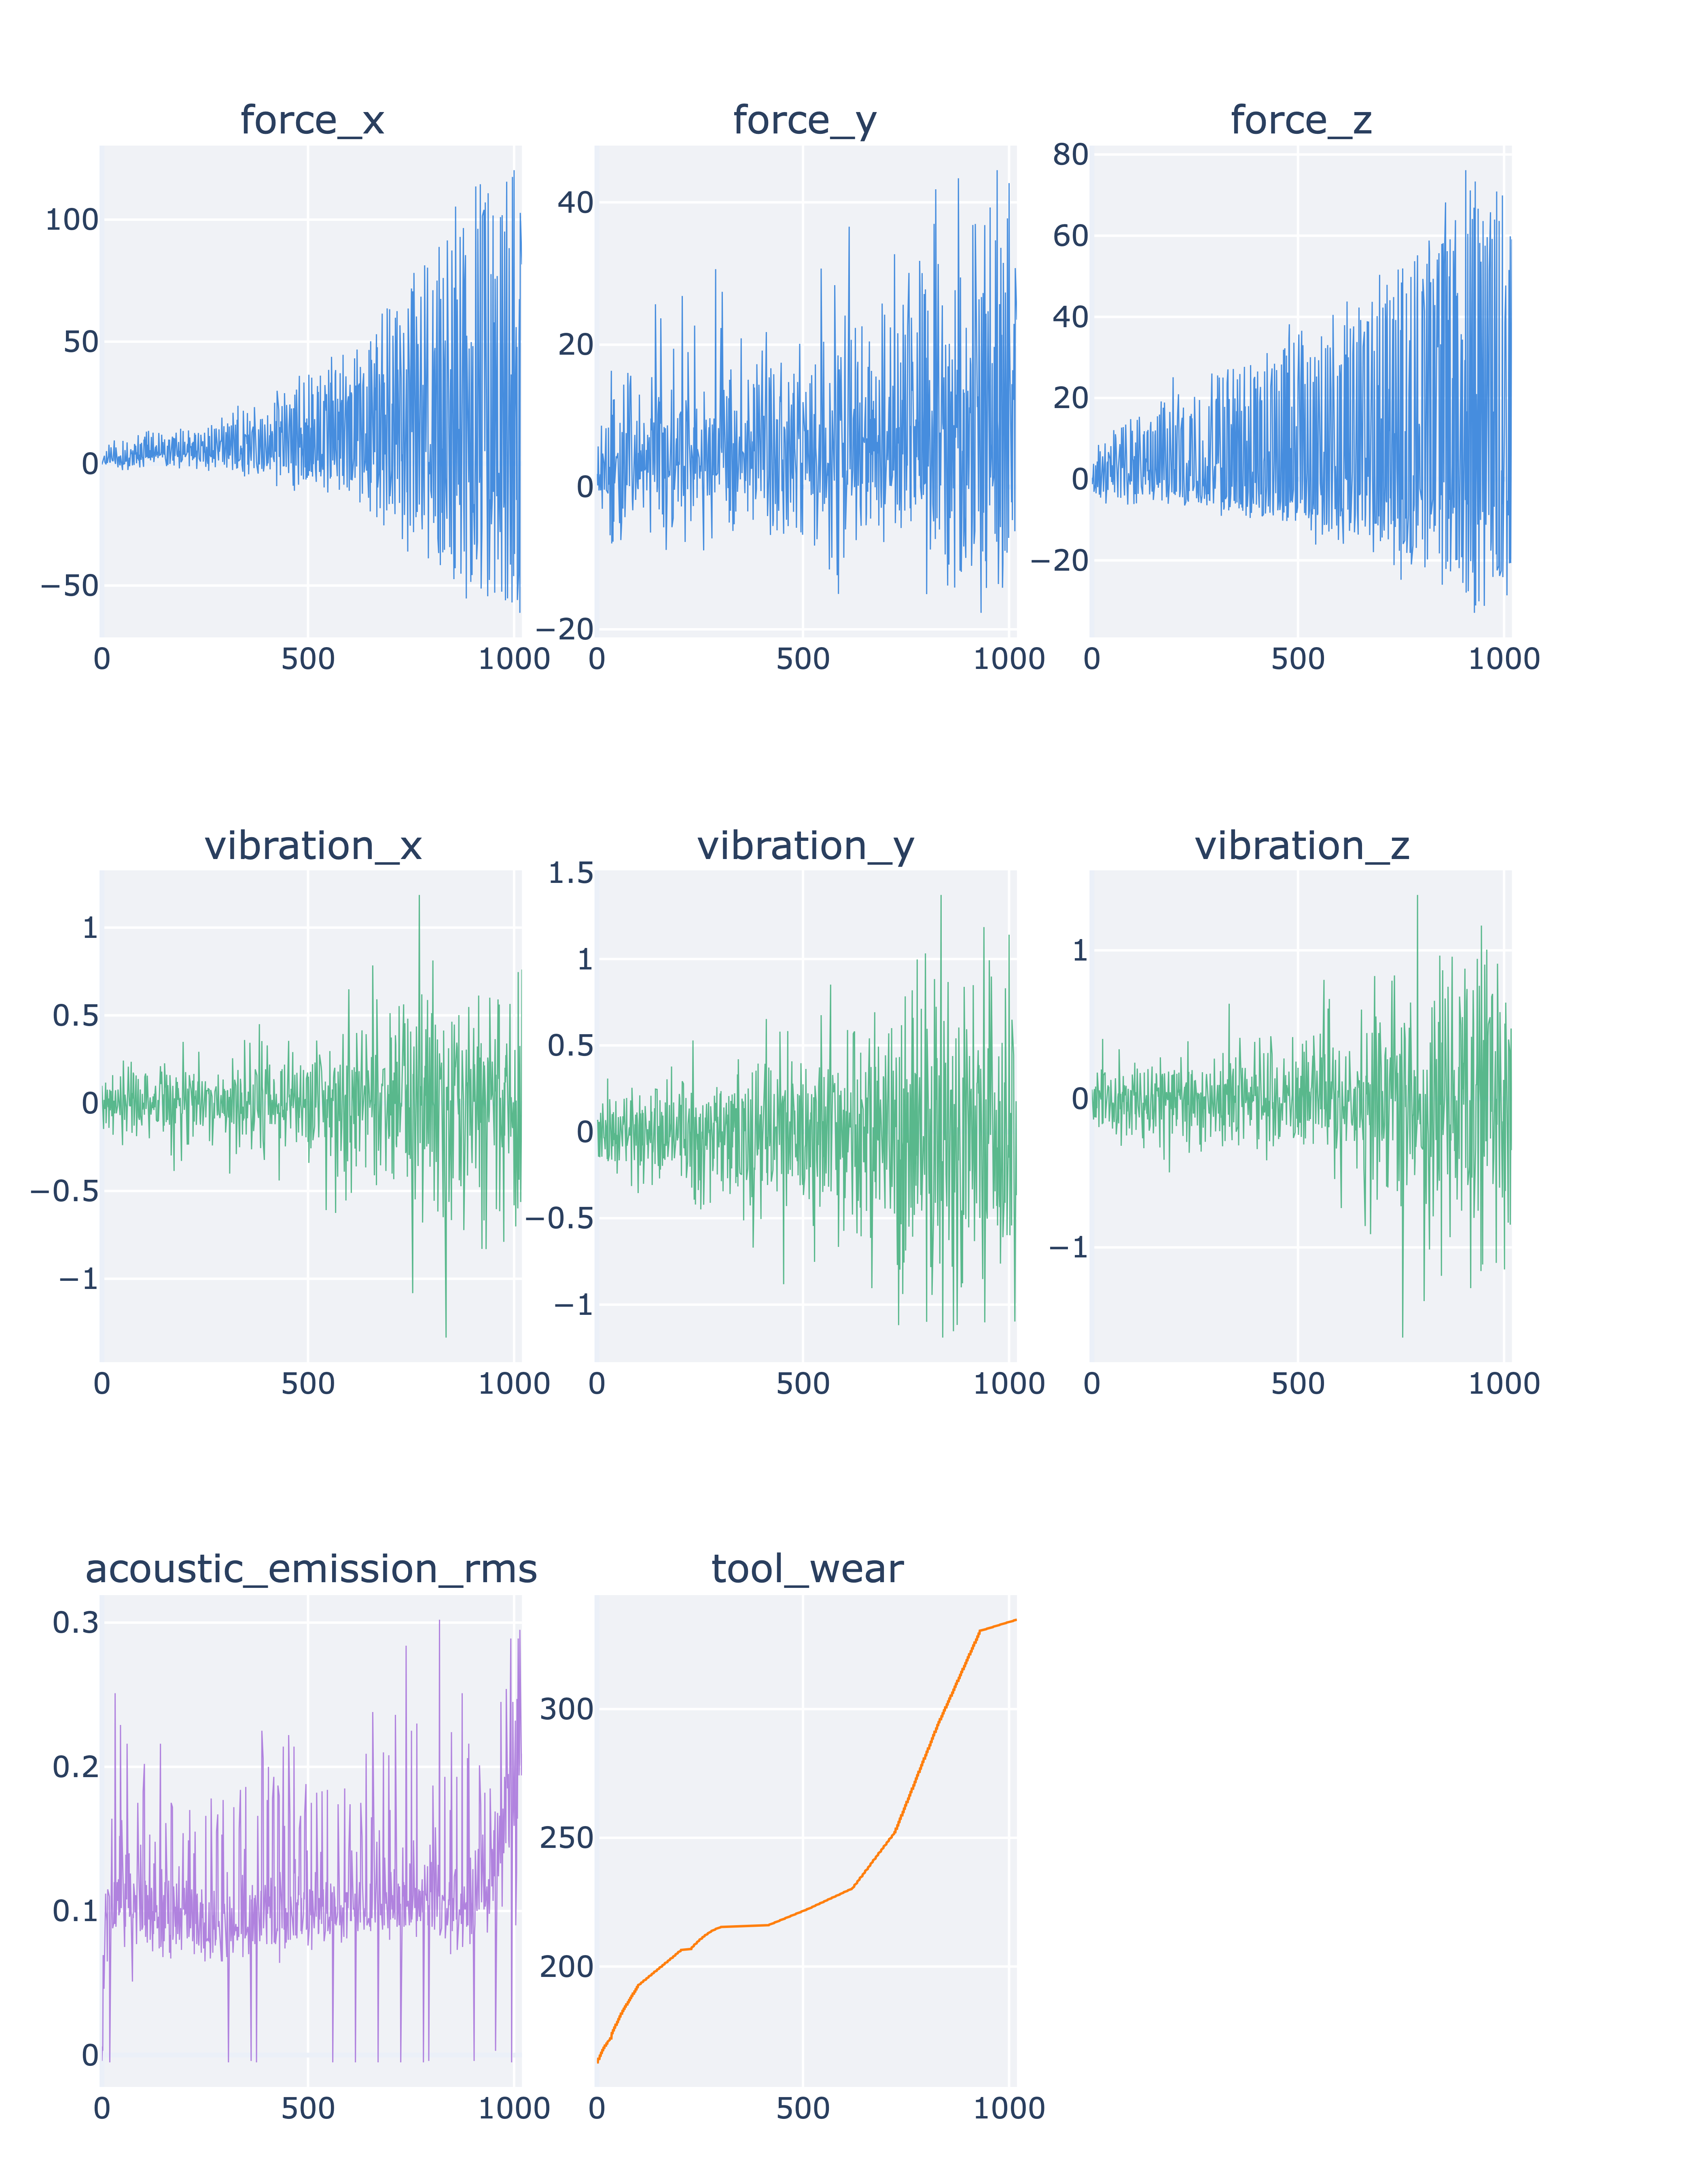
\includegraphics[width=\linewidth]{IEEE_06_SensorPlot.png}
		\caption{IEEE schema features.}
		\label{fig:schema_ieee}
	\end{subfigure}\hfill
	\begin{subfigure}[t]{0.48\textwidth}
		\centering
		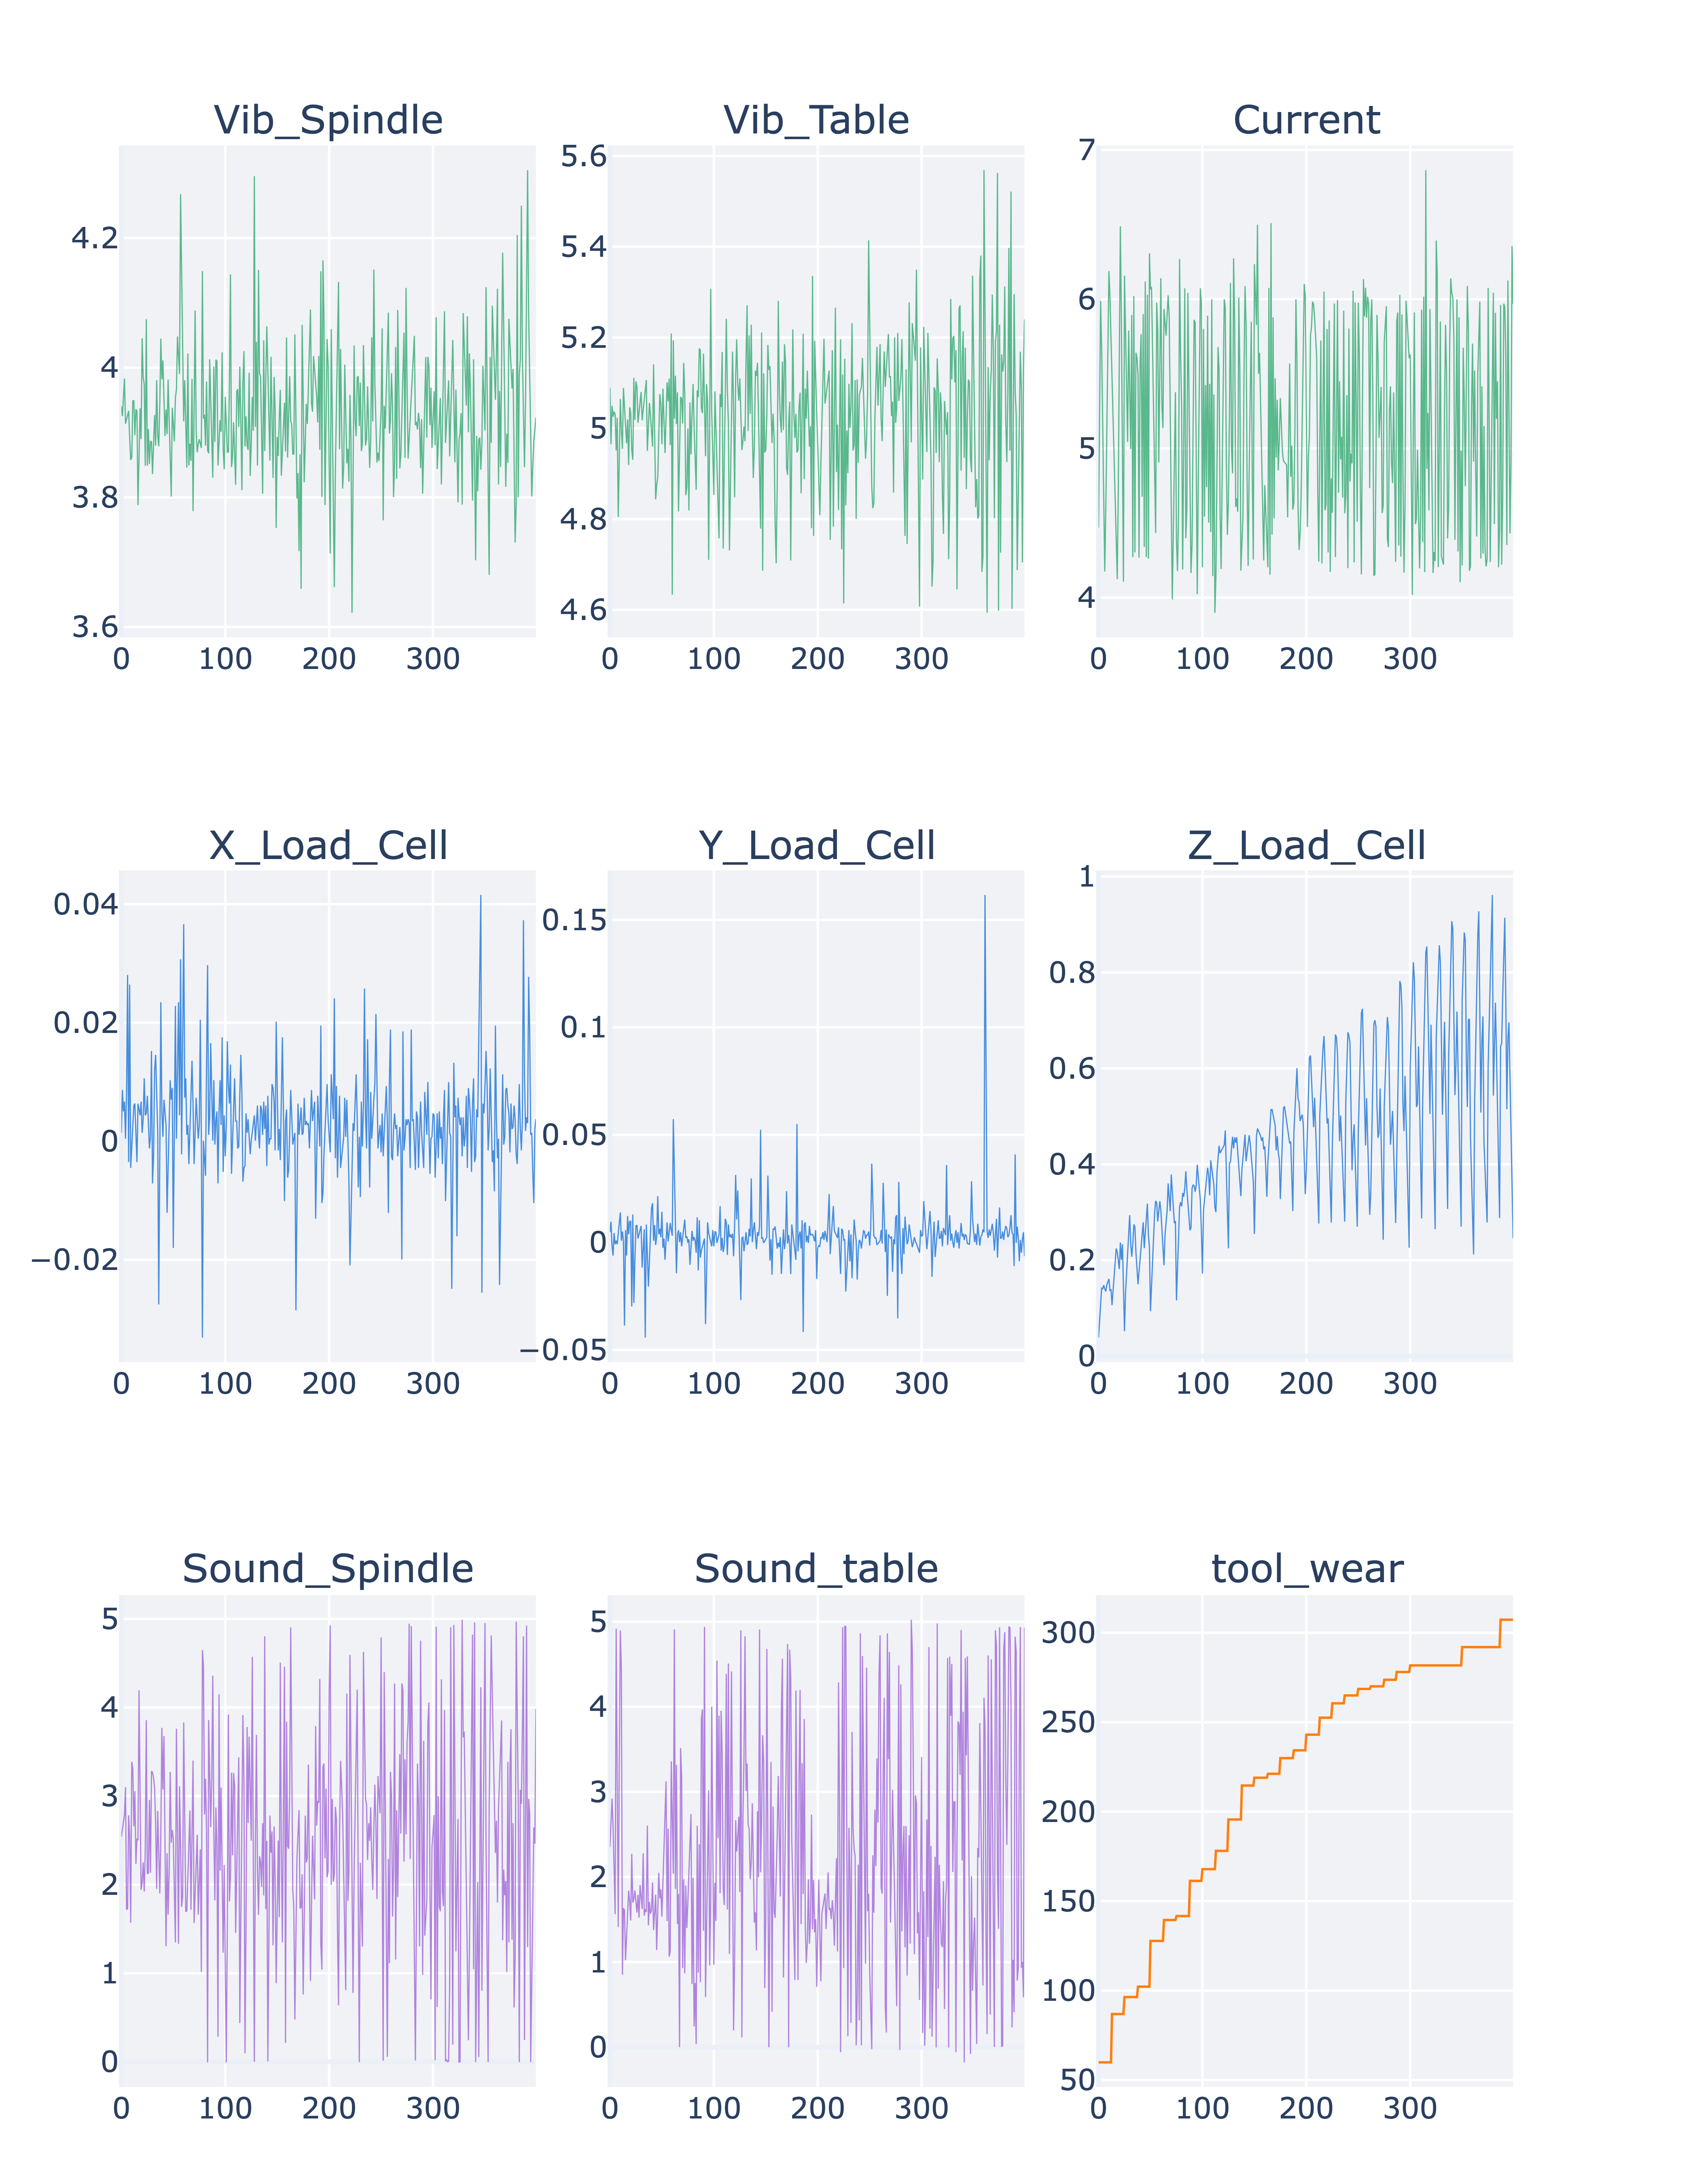
\includegraphics[width=\linewidth]{SIT_20_SensorPlot.png}
		\caption{SIT schema features.}
		\label{fig:schema_sit}
	\end{subfigure}

	\caption{Representative IEEE and SIT sensor traces showing schema differences.}
	\label{fig:schema_feature_plots_ieee_sit}
\end{figure}

\textbf{Differences between schemas:}
The schemas differ in channel count and sensor type. IEEE uses force, vibration, and acoustic emission; SIT uses vibration, sound, load, and current. The environment changes only the sensor set.

\paragraph{Datasets and train/test protocol:}
Each model is trained on one wear-cycle file and evaluated on the remaining unseen files from the same schema. SIT is the main experiment; IEEE is an external schema check.

\paragraph{Baselines and metrics:}
\label{sec:metrics}
The main comparison is among RL agents using raw sensor observations. Conventional supervised-ML baselines are not included because they require target construction, forecasting choices, or task-specific feature engineering. This is a scope choice; non-RL baselines remain future work.

\paragraph{Evaluation metrics:}
We report evaluation score, tool usage (\%), and a $\lambda$ timing metric. SIT uses repeated stochastic evaluation per held-out file; IEEE is treated as a smaller external schema check.

\paragraph{Evaluation score definition:}
Let $u\in[0,1]$ be the tool-usage fraction at first replacement, let $v\in\mathbb{N}_0$ be the number of post-threshold timesteps without replacement (threshold violations), and let $\lambda$ be the signed timing error defined below. The evaluation score is
\begin{align}
	S_{\text{tool}} &= u,\\
	S_{\text{tim}} &= \max\left(0,\,1-\frac{|\lambda|}{c_{\mathrm{IAR}}}\right),\\
	S_{\text{viol}} &= \frac{1}{1+v},\\
	S &= 0.50\,S_{\text{tool}} + 0.30\,S_{\text{tim}} + 0.20\,S_{\text{viol}}.
\end{align}
Here $c_{\mathrm{IAR}}$ scales $\lambda$ to a unit interval. If no replacement occurs before truncation, the episode is treated as a failure-to-replace case and the timing term receives its worst clipped value.

%% Lambda
\paragraph{Lambda metric and offline prognostic evaluation:}
Following offline prognostic evaluation ideas \cite{Saxena2010Metrics}, let $t_{\lambda}$ be the first timestep where wear exceeds the in-advance replacement (IAR) lower bound, and let $t_{\mathrm{FR}}$ be the first replacement timestep. Then
\begin{equation}
		\lambda = t_{\lambda} - t_{\mathrm{FR}}.
\end{equation}
With $t_{\tau}$ as the first timestep where wear exceeds $\tau$, we set
\begin{equation}
\qquad c_{\mathrm{IAR}} = t_{\tau}-t_{\lambda},
\end{equation}
so $S_{\text{tim}}$ penalizes timing error over the IAR window and is clipped at zero outside it.

\paragraph{Multi-round evaluation, confidence intervals, and exploratory hypothesis tests:}
SIT uses 20 evaluation rounds per held-out file to capture stochastic action variation. Welch tests are treated as exploratory because observations are nested within trained-model/held-out-file pairs. We report sample means and 95\% confidence intervals over held-out evaluations.

\section{Results} \label{sec:results}
This section reports refreshed results from the 17-Jul-2026 rerun. For each schema, four RL algorithms are evaluated with no attention (baseline) and four attention mechanisms (Nadaraya--Watson, temporal, self-attention, and multi-head).

\subsection{Main performance tables and focused statistical tests}
\label{sec:hypothesis_tests}

Tables~\ref{tab:sit_main_results} and \ref{tab:ieee_main_results} report mean $\pm$ standard deviation of evaluation score. Table~\ref{tab:rf_vs_ppo_tests} gives the focused one-tailed Welch tests for the claim \textsc{REINFORCE} $>$ \textsc{PPO}.

\begin{table}[htbp]
	\centering
	\caption{SIT schema: mean $\pm$ std. dev. evaluation score.}
	\label{tab:sit_main_results}
	\begin{tabular}{l l l l l l}
	\toprule
	\textbf{RL Algo} & \textbf{Baseline} & \textbf{NW} & \textbf{TP} & \textbf{SA} & \textbf{MH}\\
	\midrule
	A2C & 0.2456 $\pm$ 0.0043 & 0.2456 $\pm$ 0.0043 & 0.2456 $\pm$ 0.0043 & 0.3130 $\pm$ 0.2040 & 0.2456 $\pm$ 0.0043\\
	DQN & 0.2456 $\pm$ 0.0043 & 0.2456 $\pm$ 0.0043 & 0.2456 $\pm$ 0.0043 & 0.2456 $\pm$ 0.0043 & 0.2456 $\pm$ 0.0043\\
	PPO & 0.6313 $\pm$ 0.3347 & 0.7132 $\pm$ 0.3172 & 0.5771 $\pm$ 0.3337 & 0.6089 $\pm$ 0.3305 & 0.8004 $\pm$ 0.2694\\
	REINFORCE & 0.4907 $\pm$ 0.3108 & 0.8646 $\pm$ 0.2032 & 0.6406 $\pm$ 0.3355 & 0.6997 $\pm$ 0.3171 & 0.7917 $\pm$ 0.2738\\
	\bottomrule
	\end{tabular}
\end{table}

\begin{table}[htbp]
	\centering
	\caption{IEEE schema: mean $\pm$ std. dev. evaluation score.}
	\label{tab:ieee_main_results}
	\begin{tabular}{l l l l l l}
	\toprule
	\textbf{RL Algo} & \textbf{Baseline} & \textbf{NW} & \textbf{TP} & \textbf{SA} & \textbf{MH}\\
	\midrule
	A2C & 0.6880 $\pm$ 0.3098 & 0.4322 $\pm$ 0.2753 & 0.3565 $\pm$ 0.2496 & 0.2729 $\pm$ 0.1281 & 0.7424 $\pm$ 0.2695\\
	DQN & 0.6696 $\pm$ 0.3002 & 0.2360 $\pm$ 0.0016 & 0.2360 $\pm$ 0.0016 & 0.2360 $\pm$ 0.0016 & 0.2878 $\pm$ 0.1811\\
	PPO & 0.8434 $\pm$ 0.1604 & 0.8343 $\pm$ 0.1867 & 0.7608 $\pm$ 0.2641 & 0.8044 $\pm$ 0.2174 & 0.8232 $\pm$ 0.1870\\
	REINFORCE & 0.7496 $\pm$ 0.2606 & 0.8008 $\pm$ 0.2186 & 0.8848 $\pm$ 0.0737 & 0.8860 $\pm$ 0.0708 & 0.8559 $\pm$ 0.1443\\
	\bottomrule
	\end{tabular}
\end{table}

\begin{table}[htbp]
	\centering
	\caption{Focused one-tailed Welch tests for \textsc{REINFORCE} $>$ \textsc{PPO} at $\alpha=0.05$.}
	\label{tab:rf_vs_ppo_tests}
	\begin{tabular}{l l r r l}
	\toprule
	\textbf{Schema} & \textbf{Setting} & \textbf{t-stat} & \textbf{p-value} & \textbf{Supported?}\\
	\midrule
	SIT & Baseline (no attention) & -2.9224 & 0.9980 & No\\
	SIT & With attention (pooled) & 3.1941 & 0.0007 & Yes\\
	IEEE & Baseline (no attention) & -1.3711 & 0.9100 & No\\
	IEEE & With attention (pooled) & 1.9865 & 0.0243 & Yes\\
	\bottomrule
	\end{tabular}
\end{table}

\paragraph{Result interpretation (updated):}
Without attention, \textsc{PPO} has the highest mean in both schemas (SIT: 0.6313; IEEE: 0.8434). With attention, the best overall mean shifts to \textsc{REINFORCE} (SIT: 0.7492; IEEE: 0.8569). This is consistent with the focused tests in Table~\ref{tab:rf_vs_ppo_tests}: the claim \textsc{REINFORCE} $>$ \textsc{PPO} is unsupported at baseline and supported when attention is enabled.

\subsection{Ablation study: attention versus no-attention}
\label{sec:ablation_results}

Table~\ref{tab:ablation_condensed} reports refreshed ablation outcomes from the 17-Jul-2026 run, including an algorithm-specific view for \textsc{REINFORCE} alongside the pooled comparisons.

\begin{table}[htbp]
\centering
\caption{Condensed ablation study from the 17-Jul-2026 run (one-tailed tests).}
\label{tab:ablation_condensed}
\begin{tabular}{l l r r r}
\toprule
\textbf{Schema} & \textbf{Comparison} & \textbf{No attn.} & \textbf{Attention} & \textbf{$p$ (1-tail)}\\
\midrule
SIT & \textsc{REINFORCE} only & 0.4907 & 0.7492 & 0.0000\\
IEEE & \textsc{REINFORCE} only & 0.7496 & 0.8569 & 0.0440\\
SIT & PPO + \textsc{REINFORCE}, pooled & 0.5610 & 0.7120 & 0.0000\\
IEEE & PPO + \textsc{REINFORCE}, pooled & 0.7965 & 0.8313 & 0.1757\\
SIT & All algorithms, pooled & 0.4033 & 0.4830 & 0.0000\\
IEEE & All algorithms, pooled & 0.7377 & 0.5906 & 1.0000\\
\bottomrule
\end{tabular}
\end{table}

For \textsc{REINFORCE}, attention significantly improves over the no-attention baseline in both schemas (SIT: 0.4907 to 0.7492, $p=0.0000$; IEEE: 0.7496 to 0.8569, $p=0.0440$), supporting attention interoperability across schemas for this algorithm. The PPO+\textsc{REINFORCE} subset follows the same direction: SIT improves significantly (0.5610 to 0.7120, $p=0.0000$), and IEEE trends upward, though the gain is not significant at $\alpha=0.05$ (0.7965 to 0.8313, $p=0.1757$). Pooled across all four algorithms, SIT again improves significantly (0.4033 to 0.4830, $p=0.0000$); the IEEE all-algorithm pooled comparison shows a different pattern, reflecting the already-strong no-attention baselines of \textsc{A2C} and \textsc{DQN} on IEEE (Table~\ref{tab:ieee_main_results}). Overall, attention interoperability across schemas is clearest for \textsc{REINFORCE}, holds more weakly for the PPO+\textsc{REINFORCE} subset, and remains schema-dependent once pooled across all four algorithms.

\subsection{Updated result figures}
Figures~\ref{fig:analysis_reports_jul17}--\ref{fig:ablation_ppo_rf_jul17} give the refreshed visual summaries for the 17-Jul-2026 rerun, corresponding to Tables~\ref{tab:sit_main_results}--\ref{tab:ablation_condensed}.

\begin{figure}[t]
	\centering
	\begin{subfigure}[t]{0.48\textwidth}
		\centering
		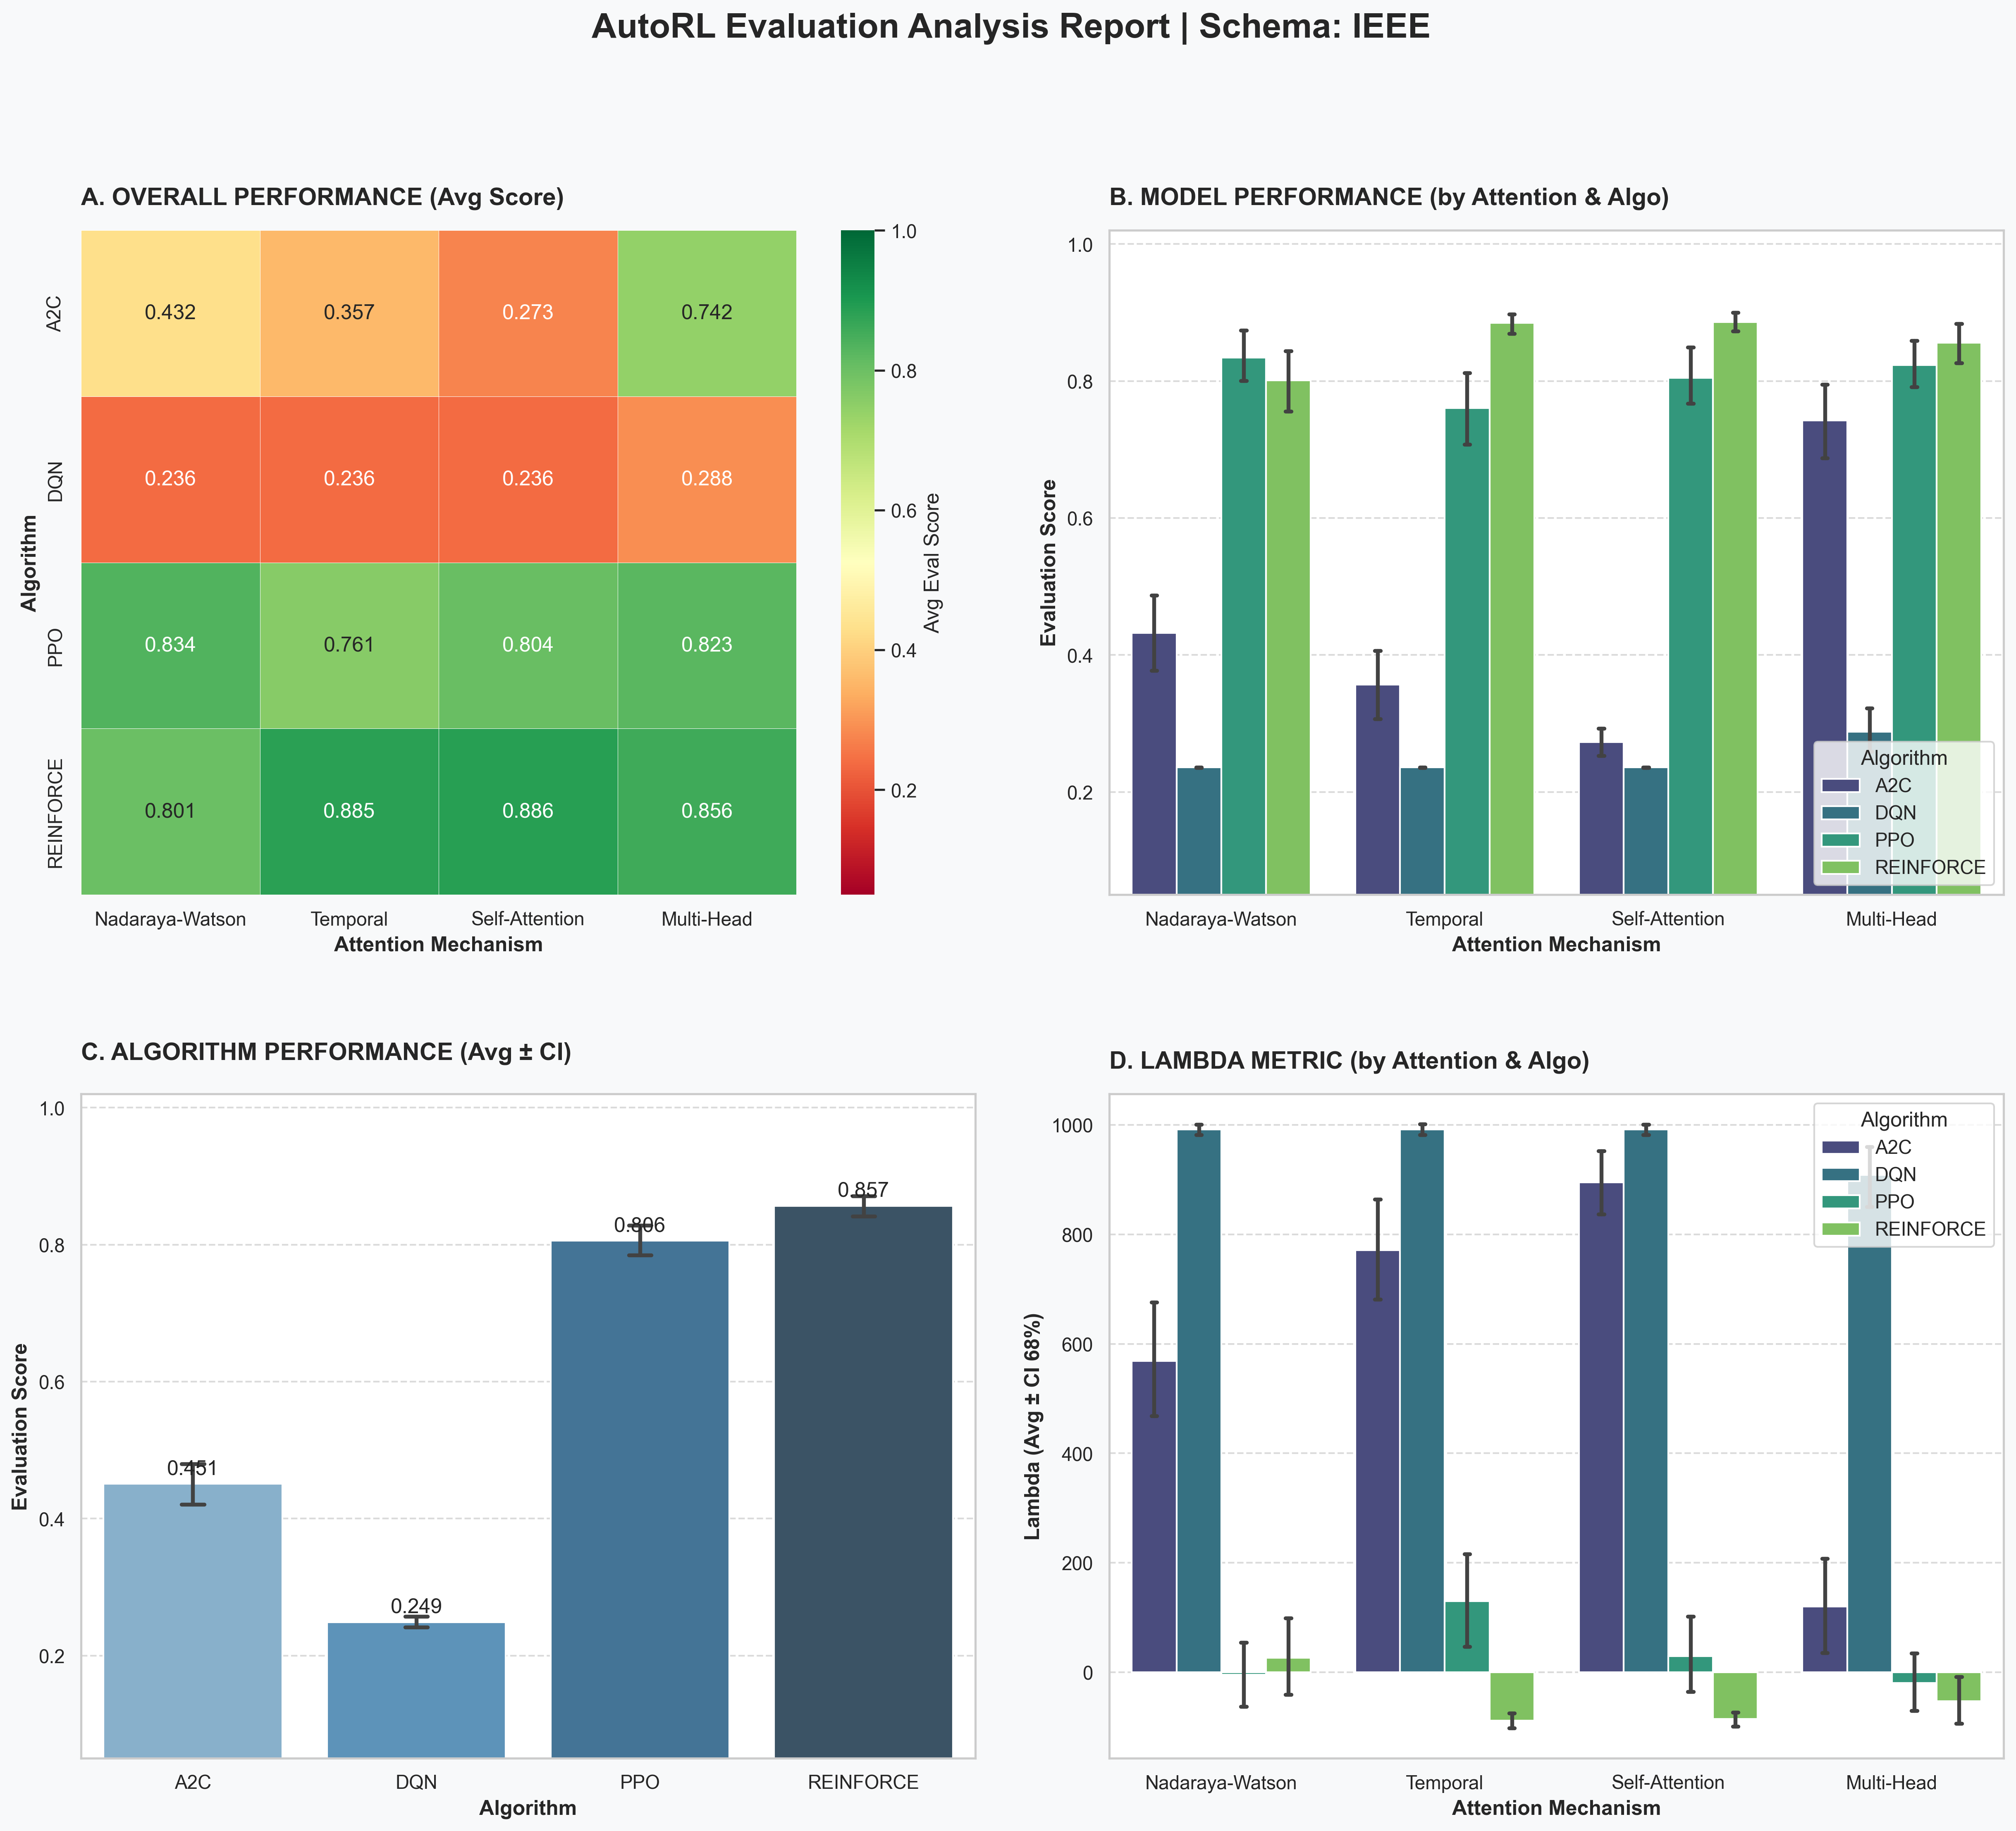
\includegraphics[width=\linewidth]{Analysis_Report_IEEE.png}
		\caption{IEEE analysis report.}
	\end{subfigure}\hfill
	\begin{subfigure}[t]{0.48\textwidth}
		\centering
		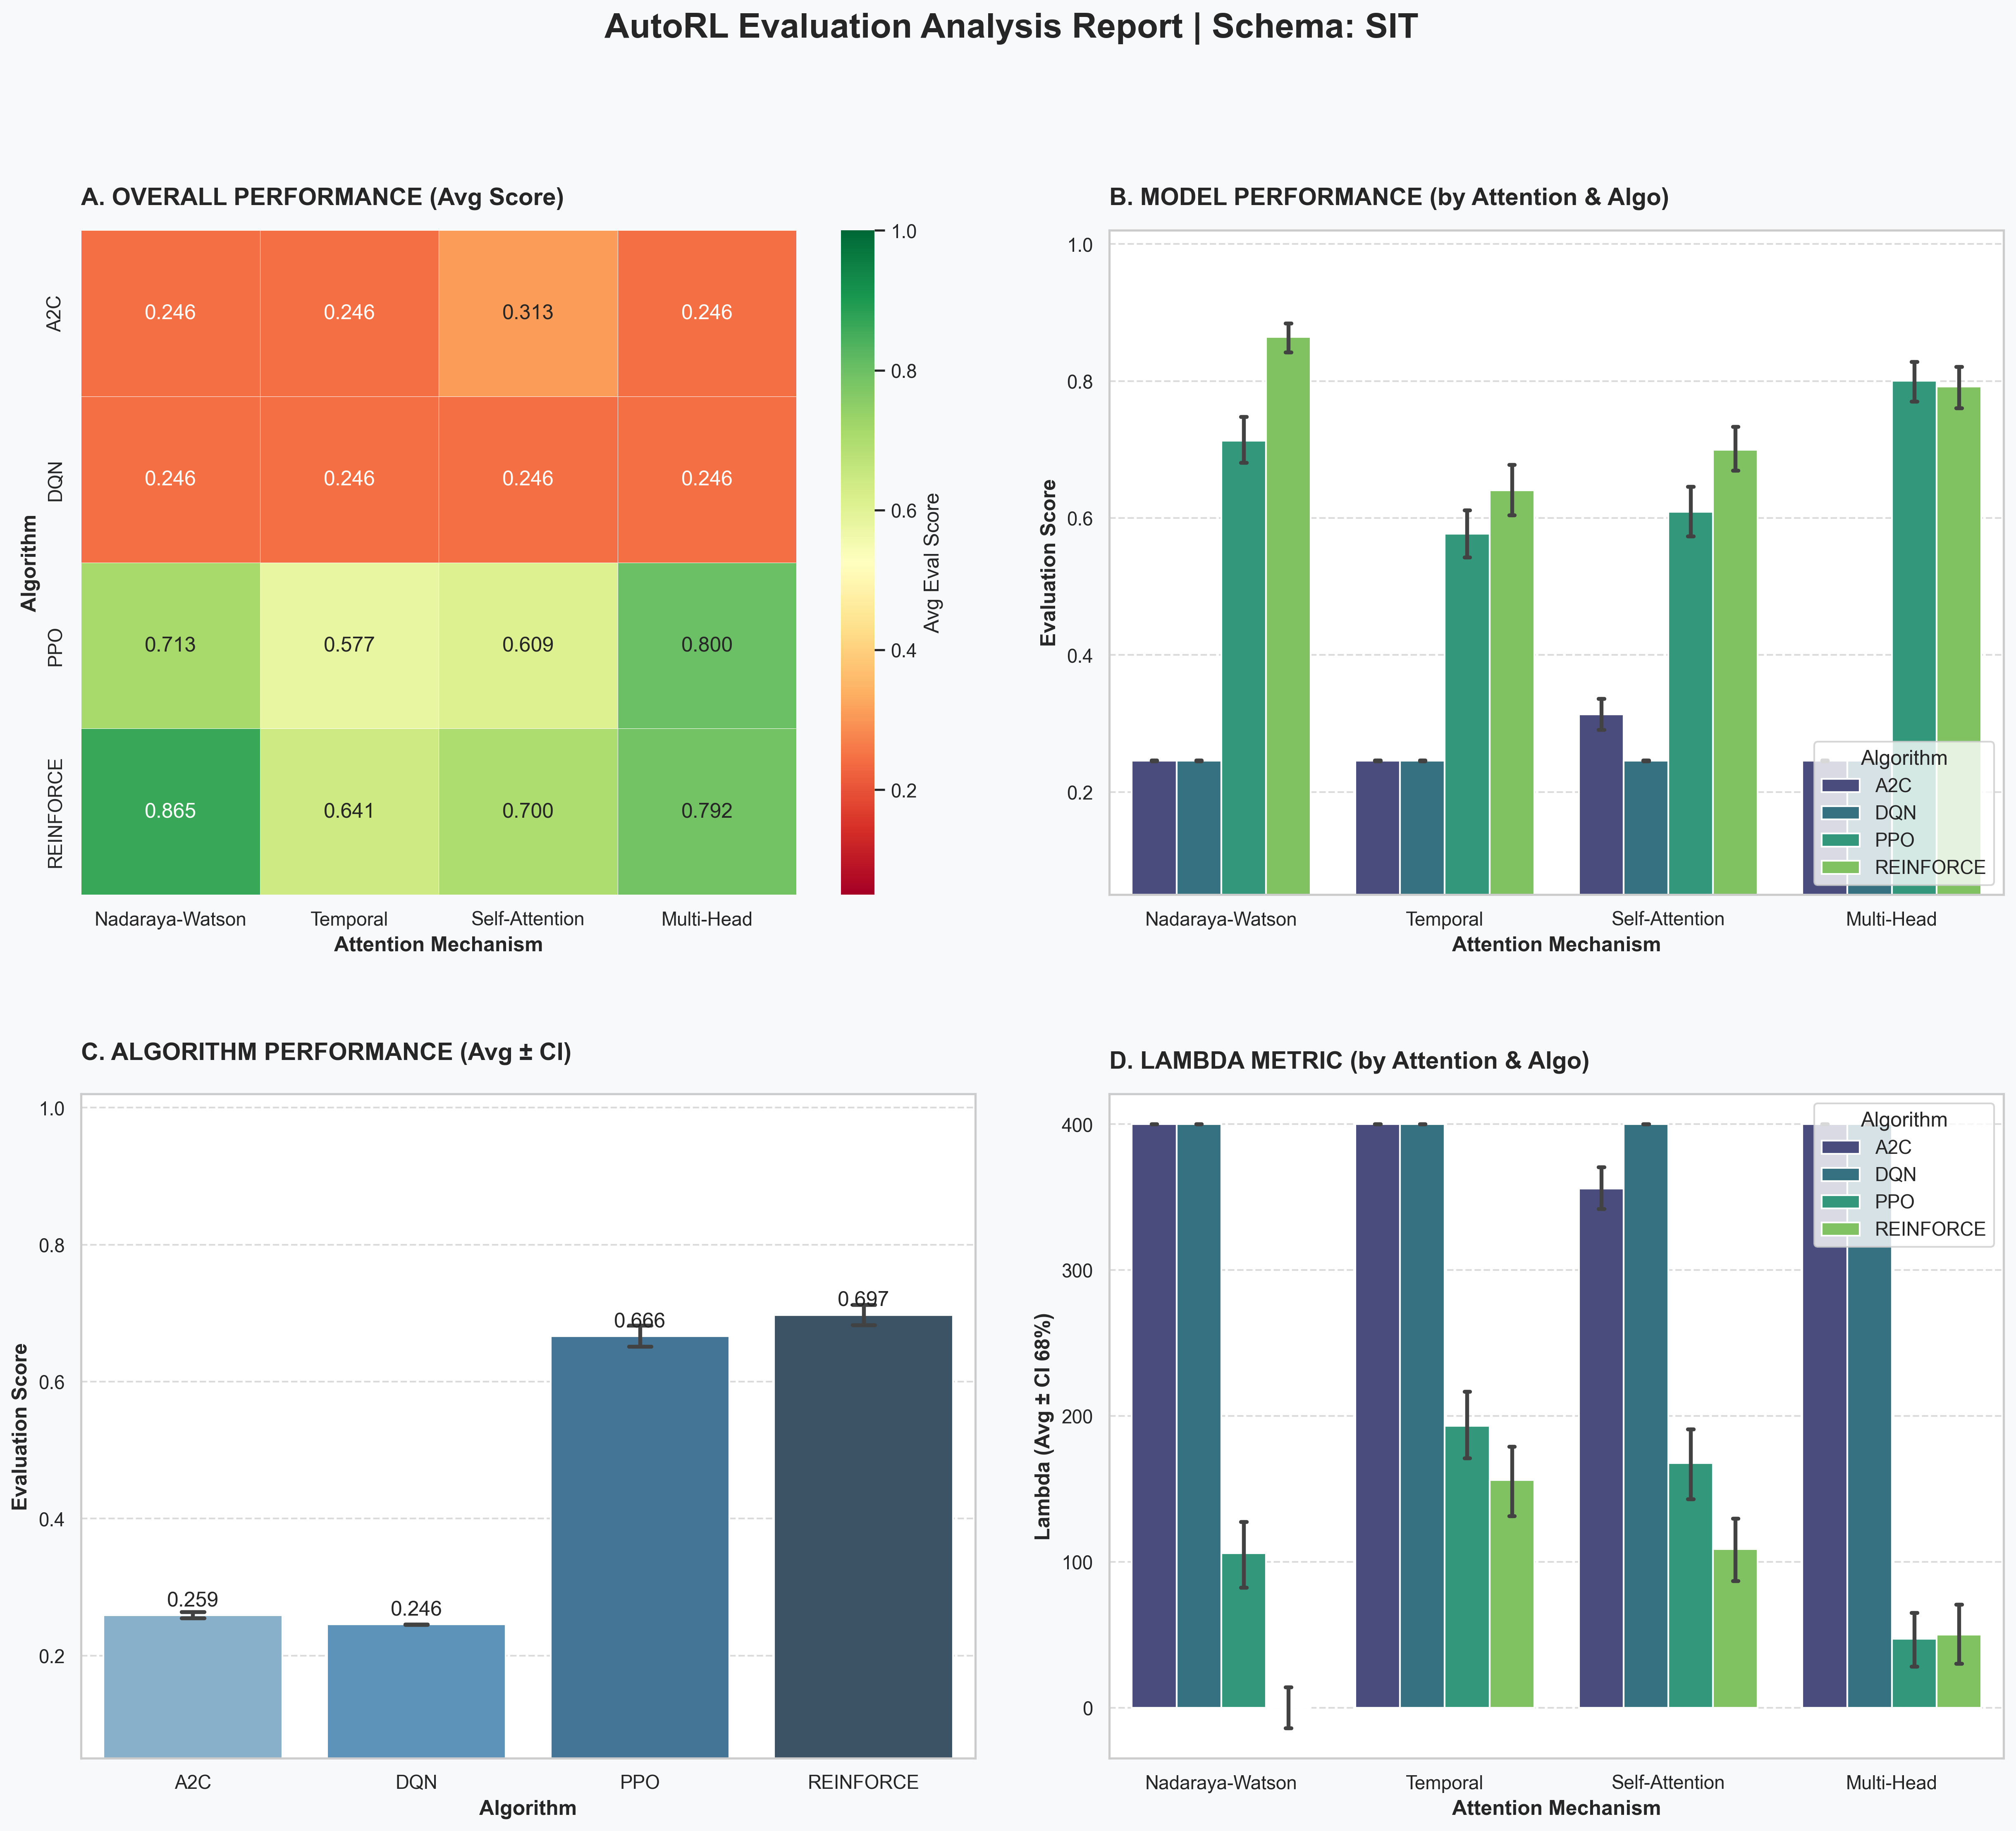
\includegraphics[width=\linewidth]{Analysis_Report_SIT.png}
		\caption{SIT analysis report.}
	\end{subfigure}
	\caption{Refreshed overall analysis reports (17-Jul-2026 run).}
	\label{fig:analysis_reports_jul17}
\end{figure}

\begin{figure}[t]
	\centering
	\begin{subfigure}[t]{0.48\textwidth}
		\centering
		\includegraphics[width=\linewidth]{Statistical_t_IEEE.png}
		\caption{IEEE $t$-statistics.}
	\end{subfigure}\hfill
	\begin{subfigure}[t]{0.48\textwidth}
		\centering
		\includegraphics[width=\linewidth]{Statistical_t_SIT.png}
		\caption{SIT $t$-statistics.}
	\end{subfigure}
	\caption{Refreshed test statistics for pairwise comparisons.}
	\label{fig:t_stats_jul17}
\end{figure}

\begin{figure}[t]
	\centering
	\begin{subfigure}[t]{0.48\textwidth}
		\centering
		\includegraphics[width=\linewidth]{Statistical_p-value_IEEE.png}
		\caption{IEEE $p$-values.}
	\end{subfigure}\hfill
	\begin{subfigure}[t]{0.48\textwidth}
		\centering
		\includegraphics[width=\linewidth]{Statistical_p-value_SIT.png}
		\caption{SIT $p$-values.}
	\end{subfigure}
	\caption{Refreshed one-tailed $p$-value plots.}
	\label{fig:p_values_jul17}
\end{figure}

\begin{figure}[t]
	\centering
	\begin{subfigure}[t]{0.48\textwidth}
		\centering
		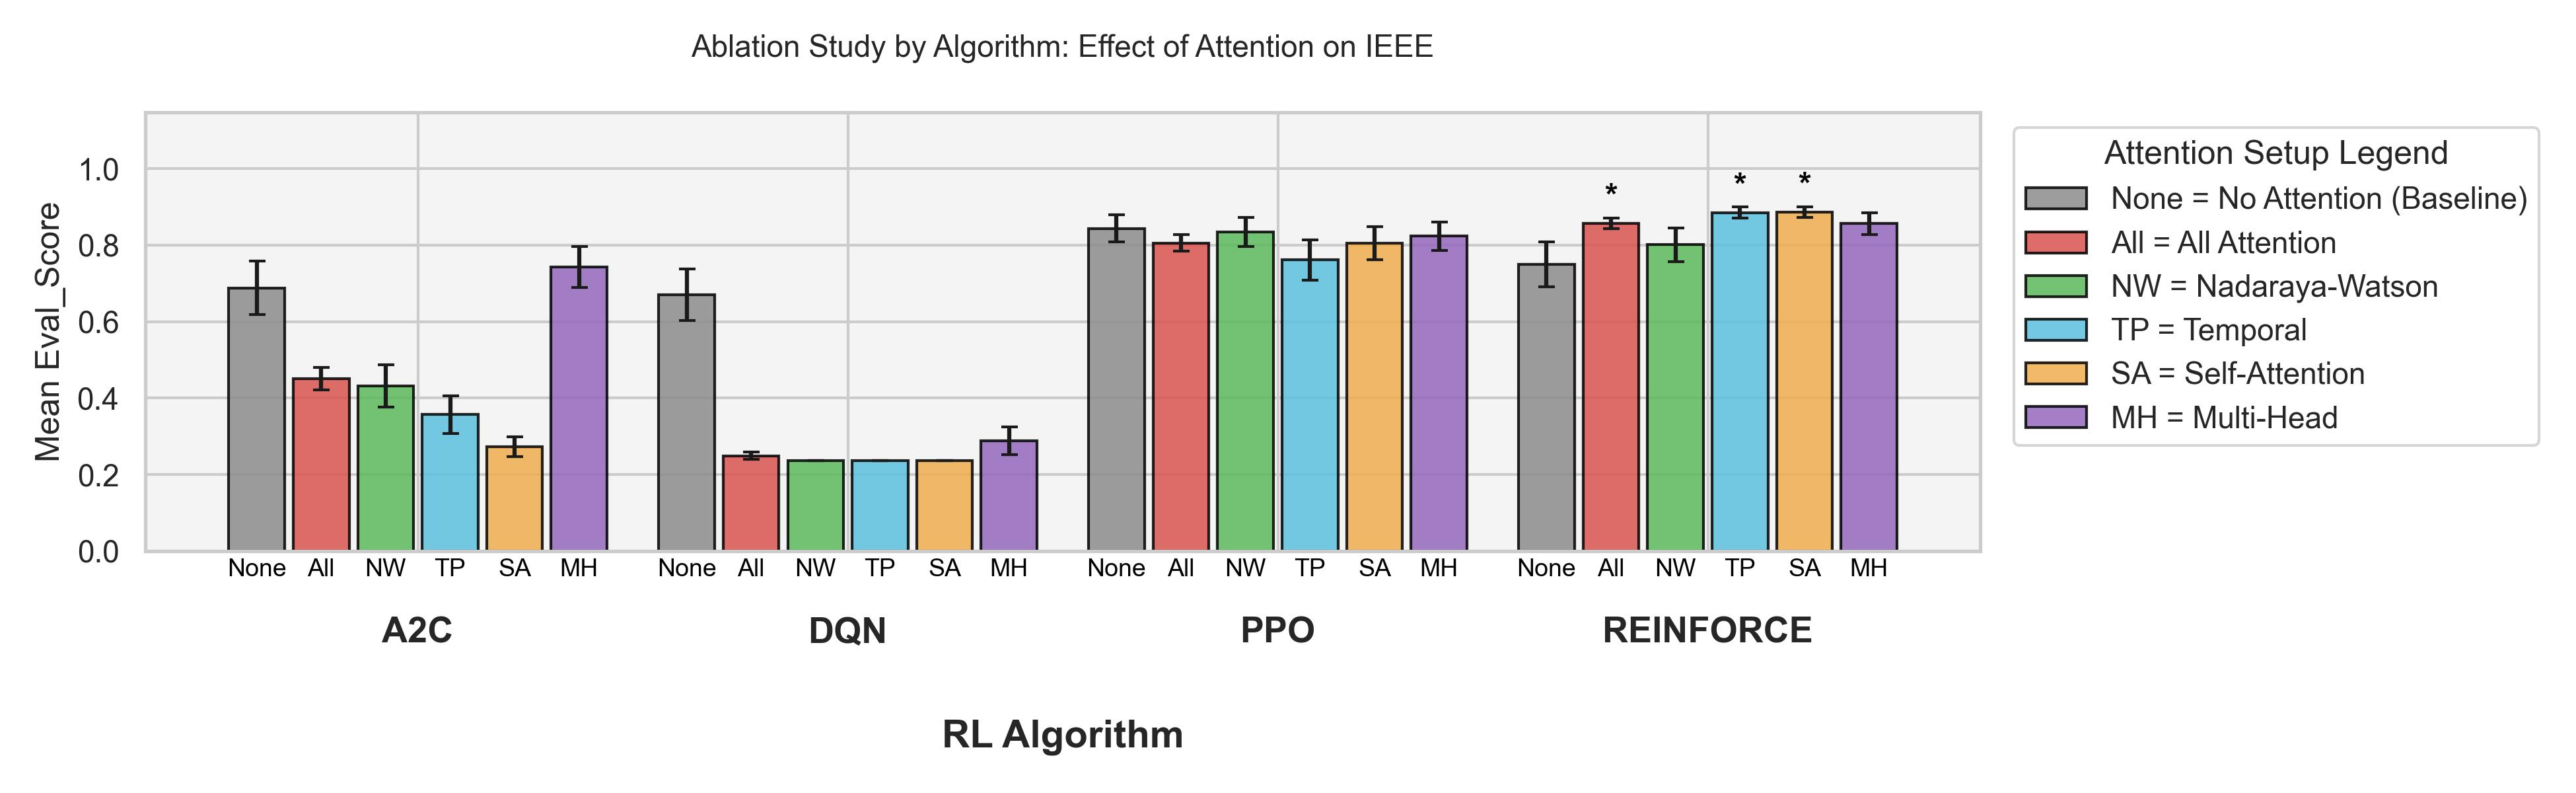
\includegraphics[width=\linewidth]{Ablation_Study_Algo_IEEE.jpg}
		\caption{IEEE ablation by algorithm.}
	\end{subfigure}\hfill
	\begin{subfigure}[t]{0.48\textwidth}
		\centering
		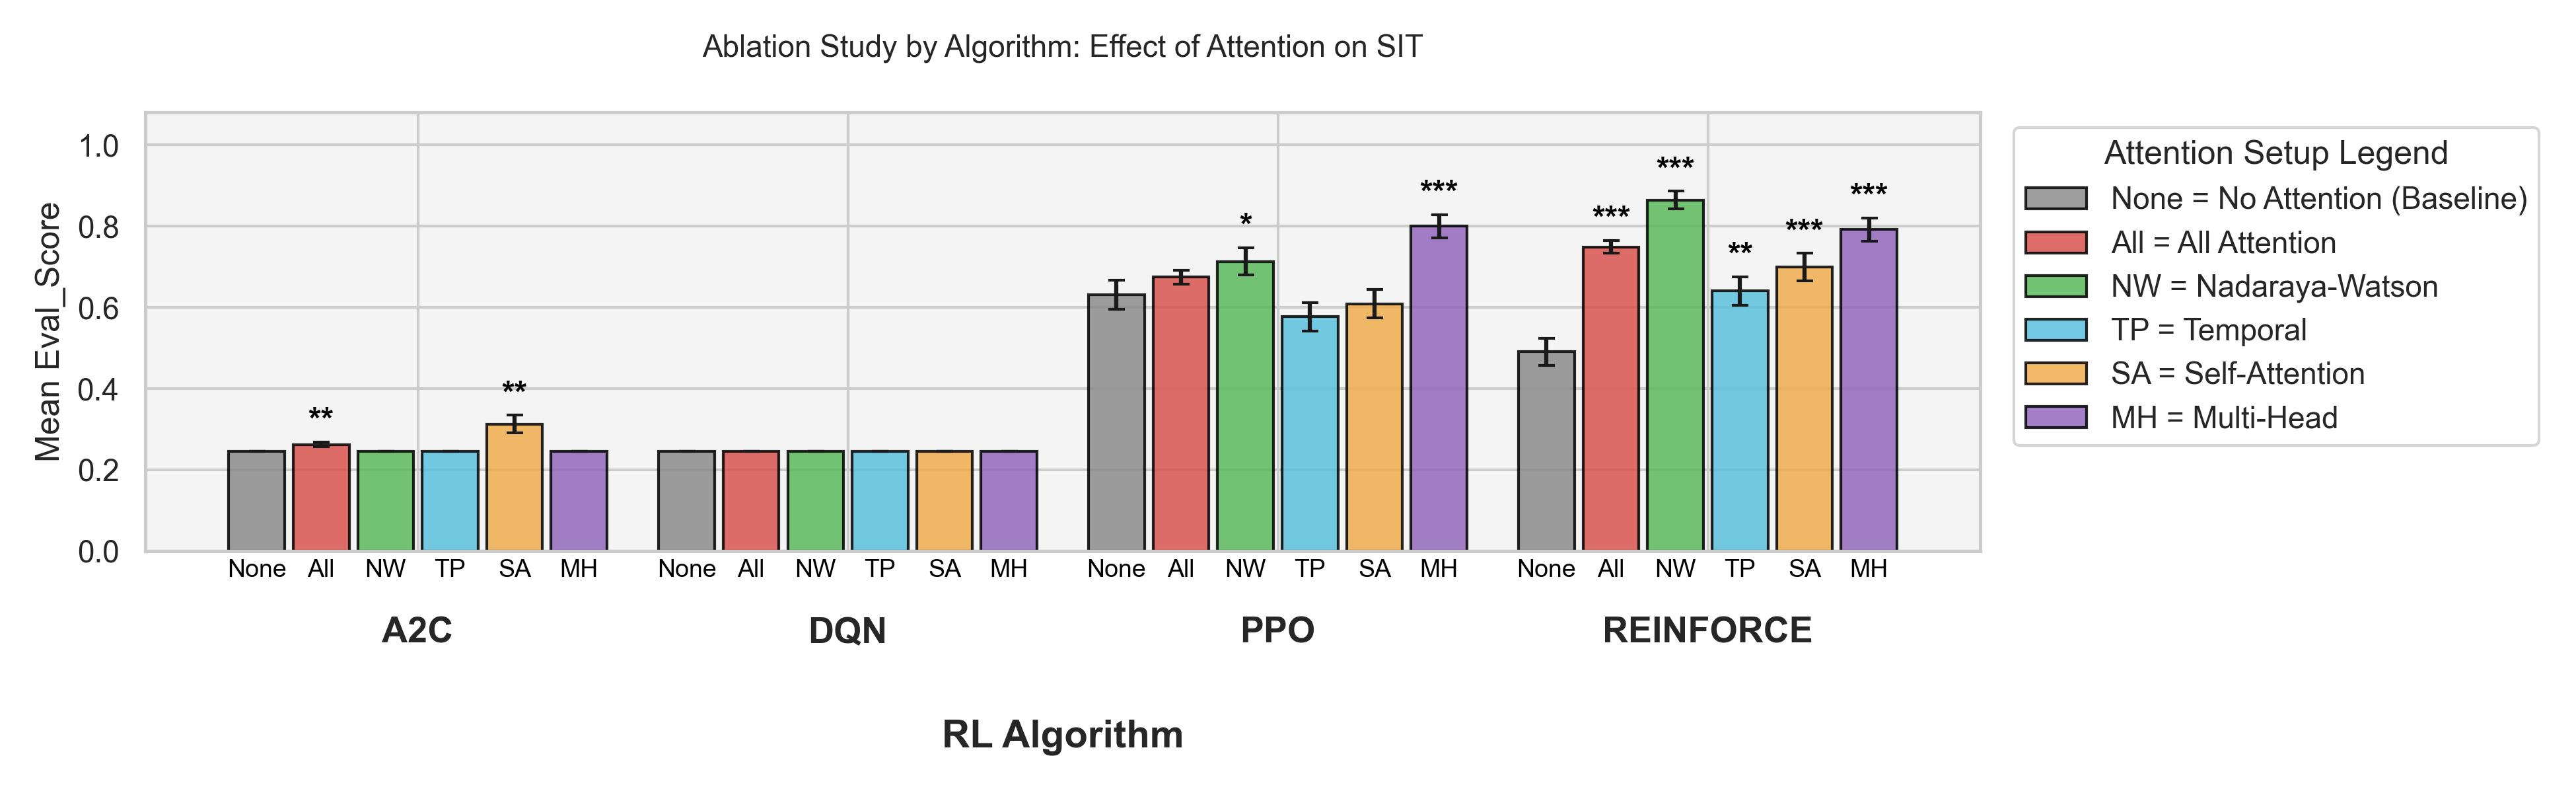
\includegraphics[width=\linewidth]{Ablation_Study_Algo_SIT.jpg}
		\caption{SIT ablation by algorithm.}
	\end{subfigure}
	\caption{Algorithm-level ablation summaries from the refreshed run.}
	\label{fig:ablation_algo_jul17}
\end{figure}

\begin{figure}[t]
	\centering
	\begin{subfigure}[t]{0.48\textwidth}
		\centering
		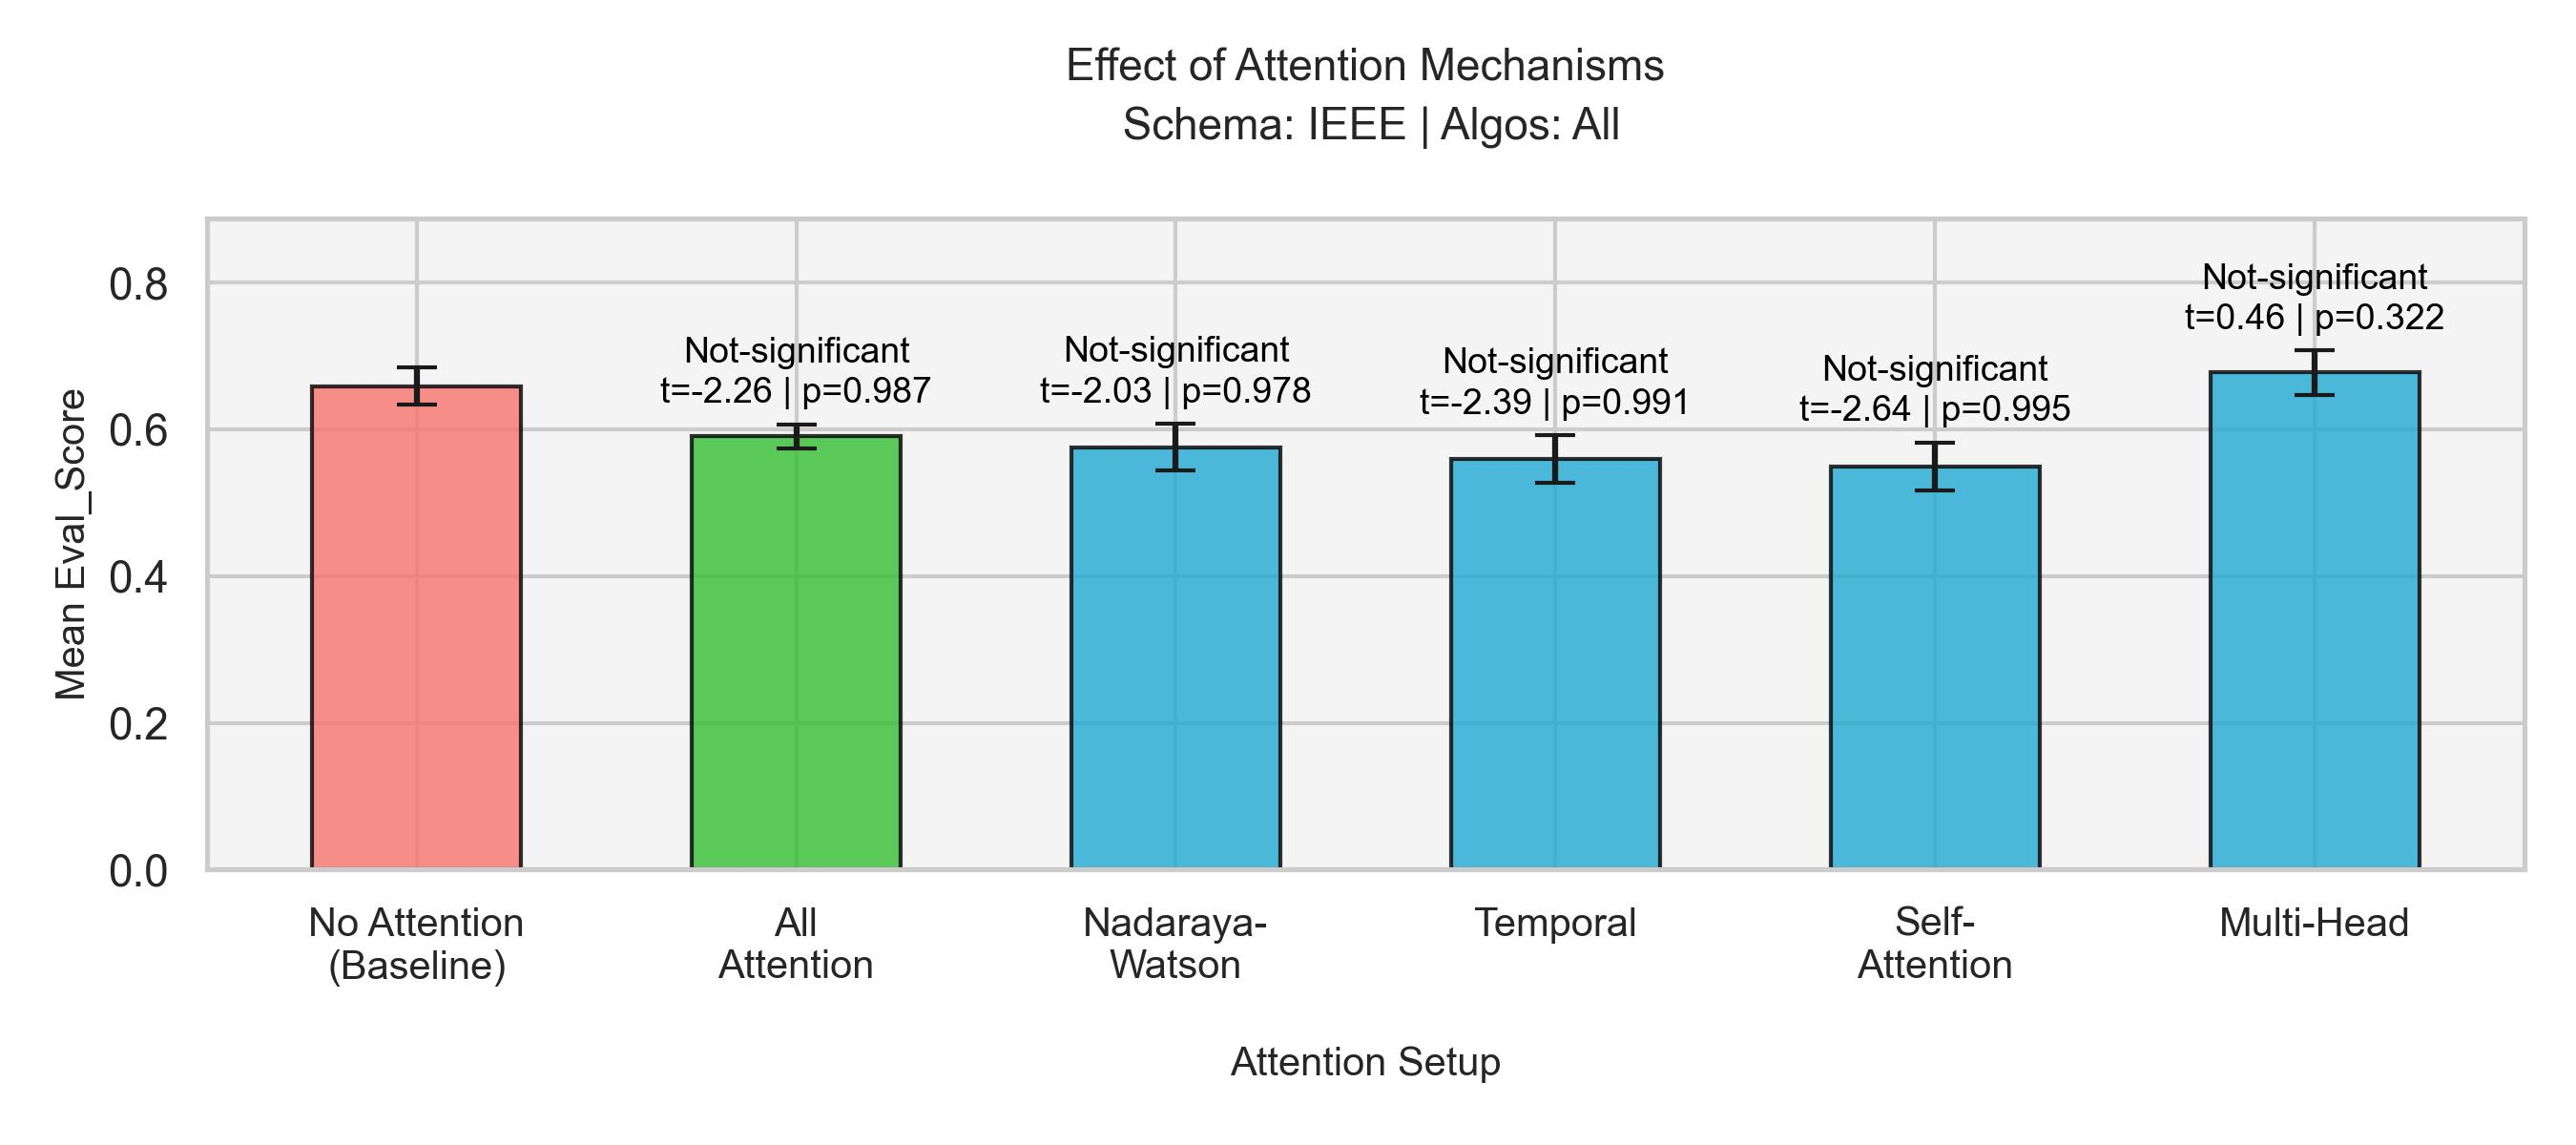
\includegraphics[width=\linewidth]{Ablation_Study_IEEE_All_Algos.jpg}
		\caption{IEEE: all algorithms pooled.}
	\end{subfigure}\hfill
	\begin{subfigure}[t]{0.48\textwidth}
		\centering
		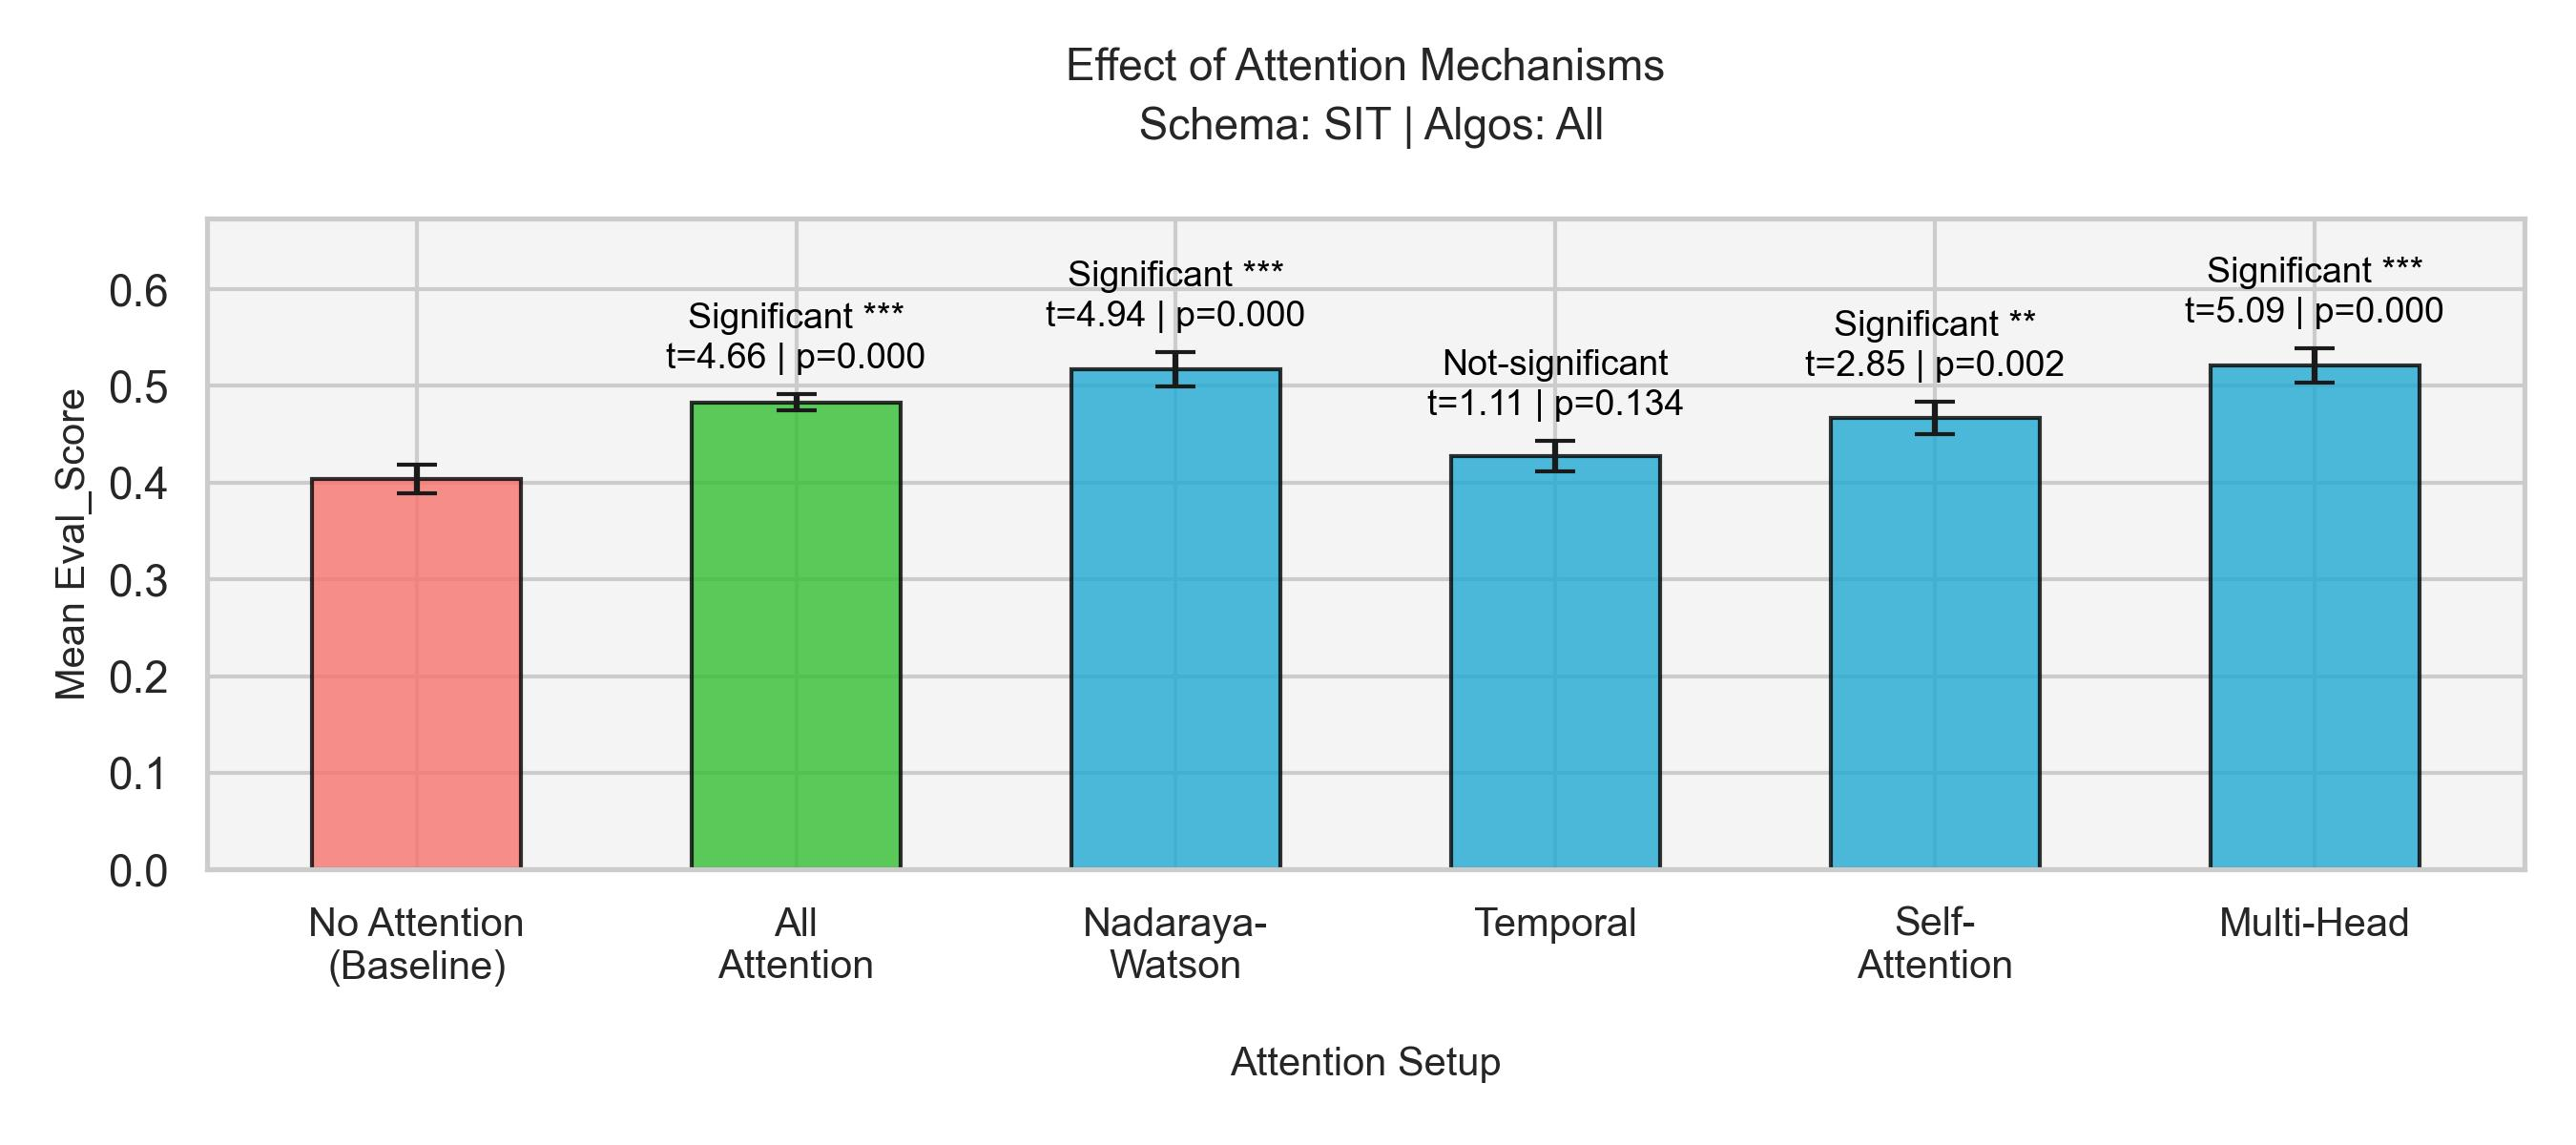
\includegraphics[width=\linewidth]{Ablation_Study_SIT_All_Algos.jpg}
		\caption{SIT: all algorithms pooled.}
	\end{subfigure}
	\caption{All-algorithm pooled ablation comparisons.}
	\label{fig:ablation_all_jul17}
\end{figure}

\begin{figure}[t]
	\centering
	\begin{subfigure}[t]{0.48\textwidth}
		\centering
		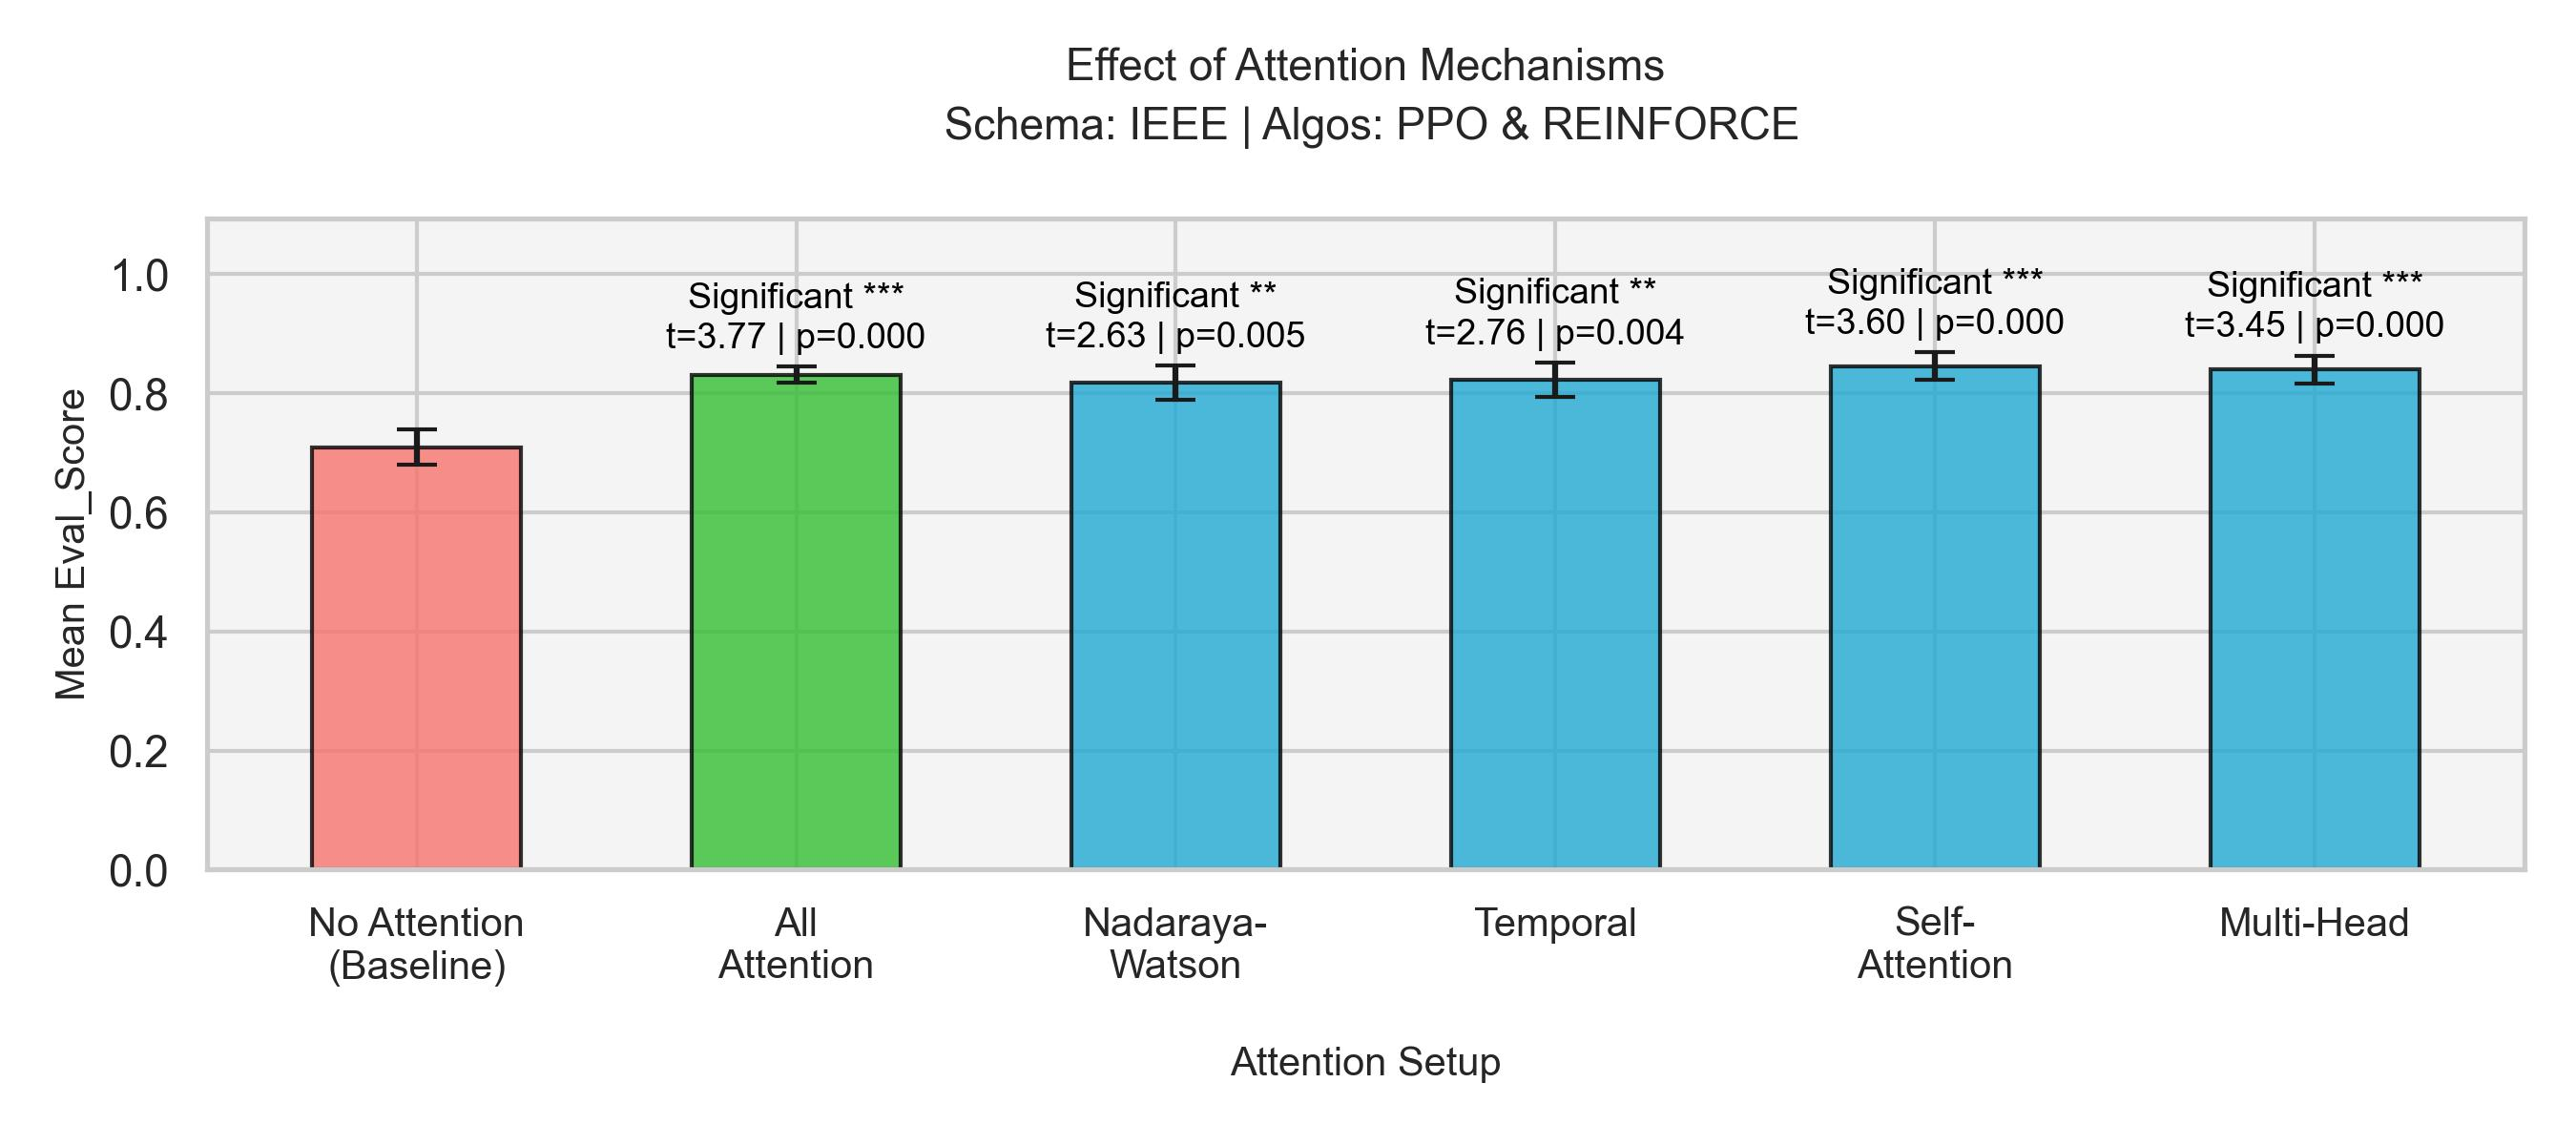
\includegraphics[width=\linewidth]{Ablation_Study_IEEE_PPO_REINFORCE.jpg}
		\caption{IEEE: PPO + \textsc{REINFORCE}.}
	\end{subfigure}\hfill
	\begin{subfigure}[t]{0.48\textwidth}
		\centering
		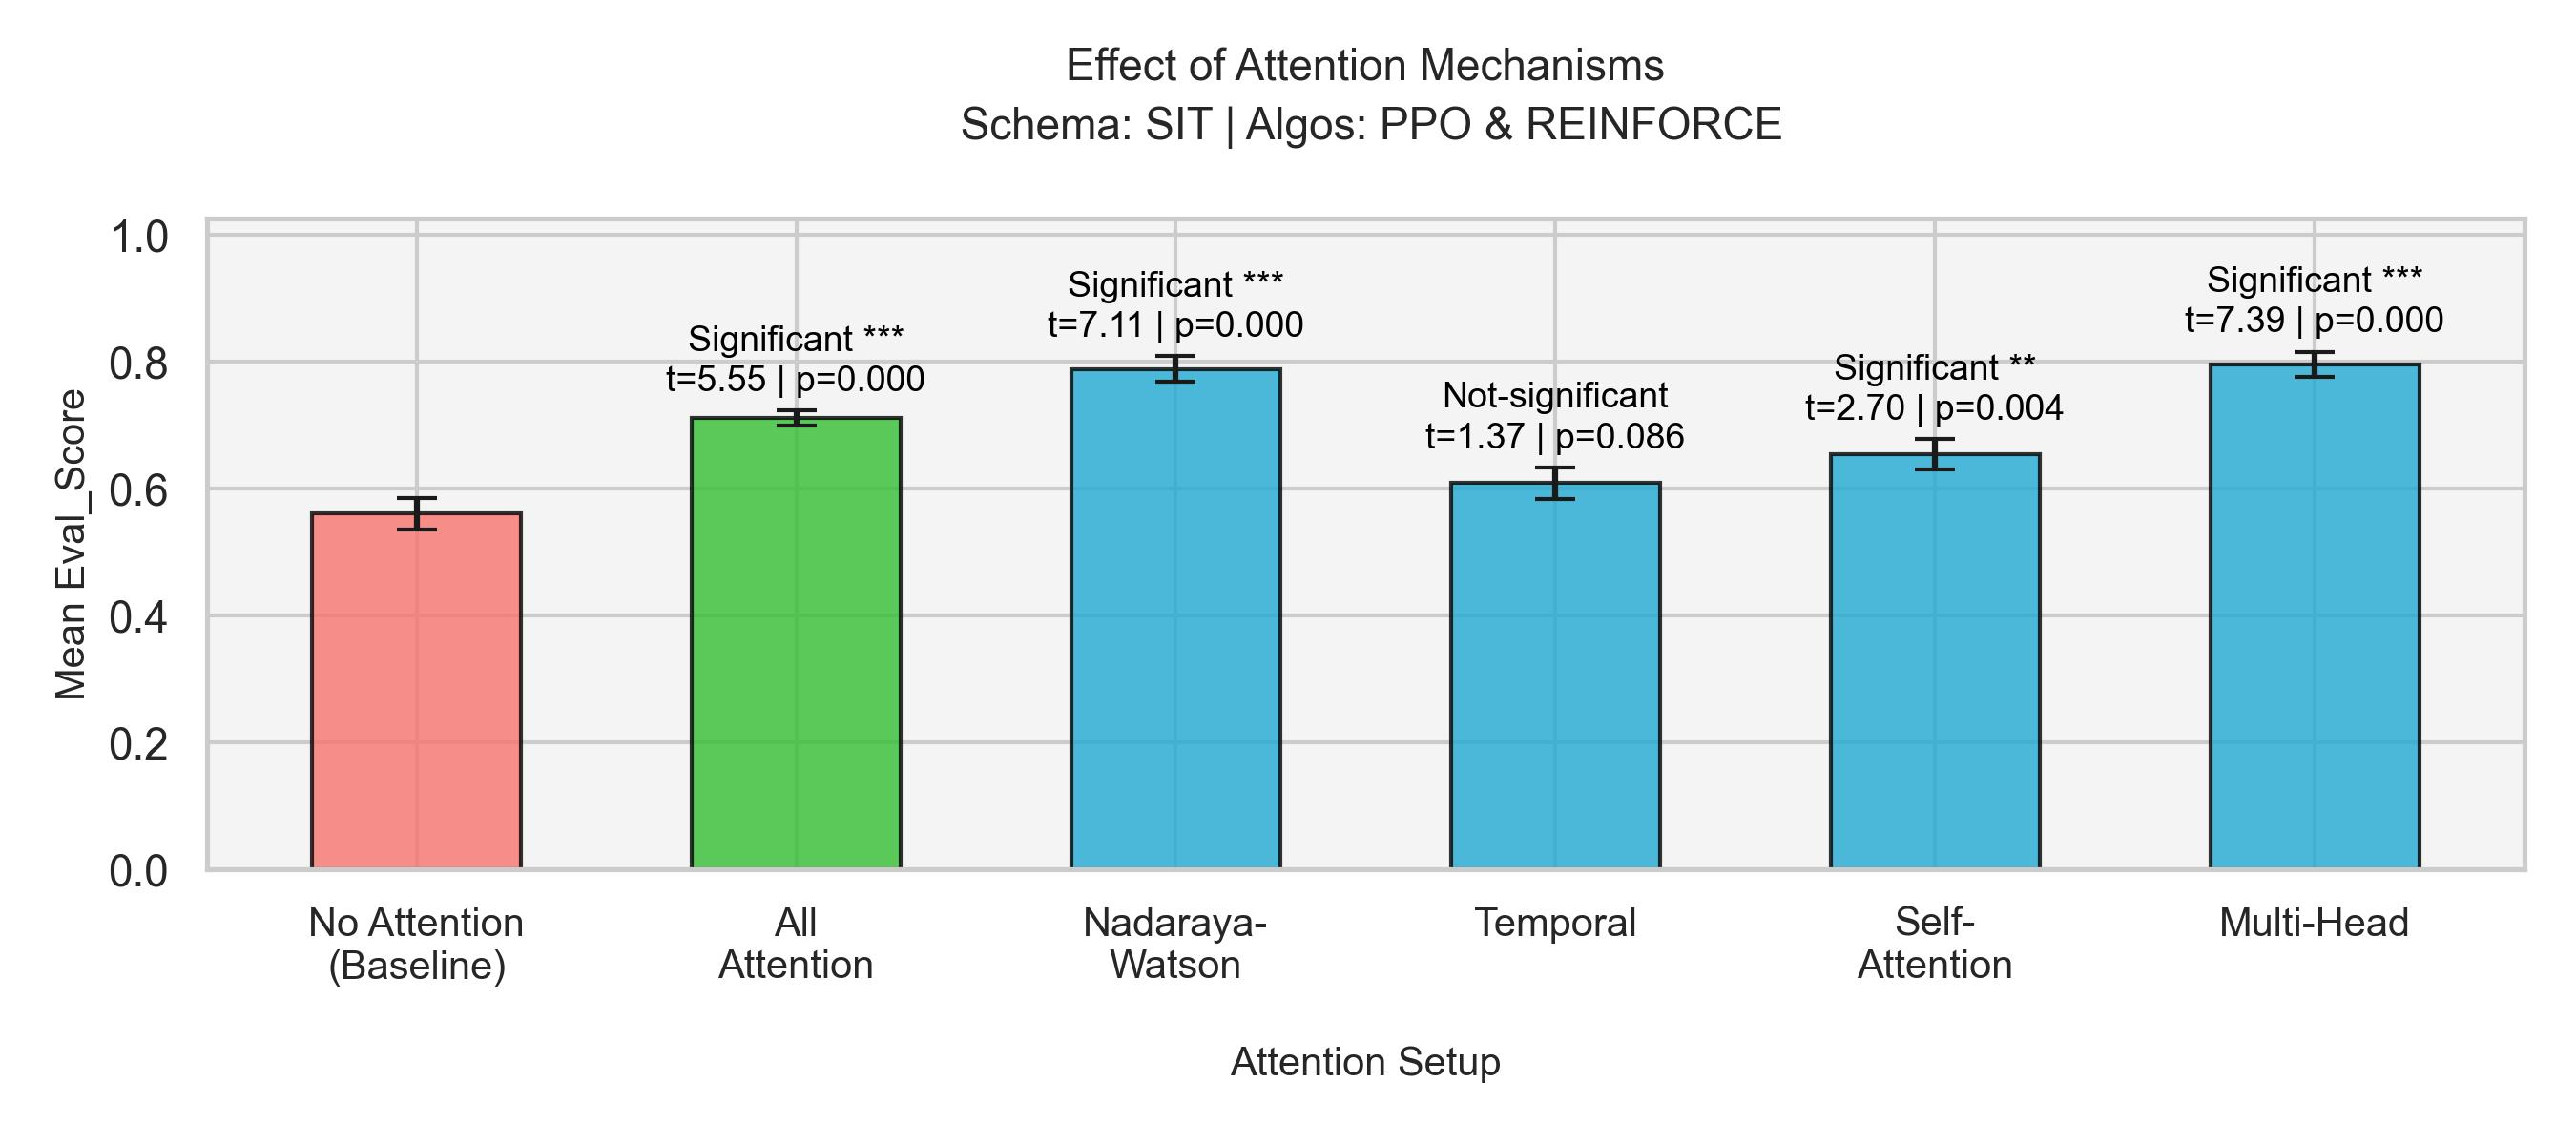
\includegraphics[width=\linewidth]{Ablation_Study_SIT_PPO_REINFORCE.jpg}
		\caption{SIT: PPO + \textsc{REINFORCE}.}
	\end{subfigure}
	\caption{Ablation comparisons focused on PPO and \textsc{REINFORCE}.}
	\label{fig:ablation_ppo_rf_jul17}
\end{figure}

\subsection{Schema portability and attention sensitivity}
The same MDP and reward logic run across both schemas, supporting environment portability at the design level. However, performance patterns are different: SIT shows strong gains for selected attention setups (especially \textsc{REINFORCE} with Nadaraya--Watson and \textsc{PPO} with multi-head), while IEEE shows a narrower separation among top policy-gradient variants and weaker pooled ablation gains. This supports schema-aware model selection rather than direct policy transfer.

\subsection{Model sizes}
As a practical aside, the trained \textsc{REINFORCE} policies are also small in serialized form in these experiments (Table~\ref{tab:model_size_summary}). This table is not a hardware-deployment study; it only reports saved model sizes.

\begin{table}[htbp]
\centering
\caption{Average serialized policy size (kB), averaged over models within each schema.}
\label{tab:model_size_summary}
\begin{tabular}{l r r}
\toprule
	\textbf{Algorithm} & \textbf{SIT avg. (kB)} & \textbf{IEEE avg. (kB)}\\
	\midrule
	A2C & 293.55 & 292.54\\
	DQN & 419.73 & 417.72\\
	PPO & 169.90 & 169.38\\
	\textbf{REINFORCE} & \textbf{169.47} & \textbf{168.95}\\
\bottomrule
\end{tabular}
\end{table}

\section{Discussion}
\label{sec:discussion}
\subsection{Why REINFORCE performed well in this PdM setup}
The task has a small action space and ends on replacement, but the policy still has to infer timing from sensor trajectories. In this rerun, \textsc{REINFORCE} becomes the best mean performer once attention is enabled in both schemas (SIT mean with attention 0.7492, IEEE mean with attention 0.8569), whereas it does not beat \textsc{PPO} in baseline-only comparisons. This pattern indicates that representation quality is a primary driver for \textsc{REINFORCE} in this PdM setting.

\subsection{Implications for industrial practitioners}
A practical deployment lesson is to benchmark no-attention first, then add attention selectively. For SIT-like schemas, attention can provide clear gains for strong policy-gradient learners. For IEEE-like schemas, pooled attention gains are not guaranteed even when some individual mechanisms improve selected learners. Therefore, encoder choice should be treated as schema-specific model selection, validated with significance testing rather than assumed to transfer.


\section{Conclusion}
\label{sec:conclusion}
\subsection{Summary of key findings}
This paper studied \textsc{REINFORCE} with attention-style feature extractors for milling-tool replacement using refreshed 17-Jul-2026 results. Without attention, \textsc{PPO} is the best mean performer in both schemas. With attention, the best mean shifts to \textsc{REINFORCE} in both schemas. Focused Welch tests show that \textsc{REINFORCE} does not exceed \textsc{PPO} in baseline-only settings, but does so after adding attention. The same environment design works across SIT and IEEE, and attention interoperability across schemas is strongest for \textsc{REINFORCE}, which improves significantly over its no-attention baseline in both SIT (0.4907 to 0.7492, $p=0.0000$) and IEEE (0.7496 to 0.8569, $p=0.0440$). This gain is not universal, however: pooled across all four algorithms, attention does not improve mean performance on IEEE (0.7377 to 0.5906, $p=1.0000$), so encoder selection must remain schema- and algorithm-specific.

\subsection{Future work}
Future work should test attention over short time windows, measure inference time and memory use, add richer maintenance costs, compare non-RL and lightweight no-attention encoders, and study robustness under sensor drift and cross-machine shift.

\section*{Statements and Declarations}

\subsection*{Acknowledgements}
The authors thank the Symbiosis Institute of Technology, for providing access to machines and measurement instruments during the duration of the project.

\subsection*{Funding}
The authors received no specific funding for this work.

\subsection*{Conflict of interest/Competing interests}
The authors have no competing interests to declare that are relevant to the content of this article.

\subsection*{Ethics approval and consent to participate}
Not applicable

\subsection*{Data availability}
The IEEE PHM~2010 milling dataset is publicly available \cite{PHMdata2010}. The SIT dataset used in this study contains in-house experimental measurements and is available from the corresponding author upon reasonable request.

\subsection*{Code availability}
The code used to train and evaluate the agents (AutoRL pipeline and the Gymnasium environment) is available from the authors upon reasonable request.

\subsection*{Author contribution}
Rajesh Siraskar, under the guidance of Satish Kumar, conceptualized the study. Rajesh Siraskar formed the methodology, and led the implementation. Satish Kumar and Arunkumar Bongale led milling-machine setup and data gathering. Shruti Patil and Satish Kumar provided program management and contributed to the manuscript review. Ketan Kotecha and Ambarish Kulkarni led program management and funding.

\begin{appendices}

\section{Progressive tool wear images - Samples}
\begin{table}[h!]
	\centering
	\caption{Progressive tool wear. Images taken using tool-makers microscope}
	\label{tab:wearimages}
	\begin{tabular}{|r|r|c|}
	\hline
	Runs & Wear $VB_{max}\mu$m & Tool condition\\
	\hline
	 0 &   0.00 & 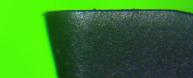
\includegraphics[width=0.3\linewidth]{tw-1.jpg} \\ \hline
	 5 & 119.71 & 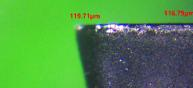
\includegraphics[width=0.3\linewidth]{tw-2.jpg} \\ \hline
	10 & 170.07 & 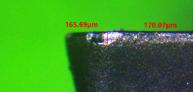
\includegraphics[width=0.3\linewidth]{tw-3.jpg} \\ \hline
	15 & 212.21 & 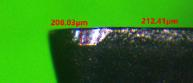
\includegraphics[width=0.3\linewidth]{tw-4.jpg} \\ \hline
	20 & 236.50 & 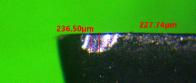
\includegraphics[width=0.3\linewidth]{tw-5.jpg} \\ \hline
	25 & 254.74 & 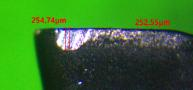
\includegraphics[width=0.3\linewidth]{tw-6.jpg} \\ \hline
	30 & 280.29 & 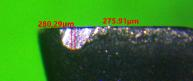
\includegraphics[width=0.3\linewidth]{tw-7.jpg} \\ \hline
	35 & 303.65 & 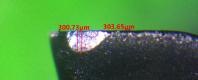
\includegraphics[width=0.3\linewidth]{tw-8.jpg} \\ \hline
	\end{tabular}
\end{table}

\end{appendices}

\clearpage
\newpage
\bibliography{references}

\end{document}